\documentclass[a4paper,10pt,twoside]{article}

\usepackage[top=1in, bottom=1in, left=1in, right=1in]{geometry}
\usepackage[utf8]{inputenc}
%\usepackage{spanish}
%\usepackage[spanish,es-ucroman,es-noquoting]{babel}
%\usepackage{setspace}
\usepackage{fancyhdr}
\usepackage{lastpage}
%\usepackage{amsmath}
%\usepackage{amsfonts}
%\usepackage{verbatim}
\usepackage{graphicx}
%\usepackage{float}
%\usepackage{algorithmic}
%\usepackage{tikz}
%\usepackage{ gensymb }
%\usetikzlibrary{calc}
%\usetikzlibrary{decorations.pathreplacing}


% Evita que el documento se estire verticalmente para ocupar
% el espacio vacío en cada página.
%\raggedbottom


%%%%%%%%%% Configuración de Fancyhdr - Inicio %%%%%%%%%%
\pagestyle{fancy}
\thispagestyle{fancy}
\lhead{TP2, Organización del Computador II}
\renewcommand{\footrulewidth}{0.4pt}
\cfoot{\thepage /\pageref{LastPage}}

\fancypagestyle{caratula} {
   \fancyhf{}
   \cfoot{\thepage /\pageref{LastPage}}
   \renewcommand{\headrulewidth}{0pt}
   \renewcommand{\footrulewidth}{0pt}
}

%%%%%%%%%% Macros de tikz - Fin %%%%%%%%%%


%%%%%%%%%% Macros misceláneos - Inicio %%%%%%%%%%
\newcommand{\xmm}[1]{\texttt{XMM#1}}
\newcommand{\rax}{\texttt{RAX}}
\newcommand{\rbx}{\texttt{RBX}}
\newcommand{\rcx}{\texttt{RCX}}
\newcommand{\rdx}{\texttt{RDX}}
\newcommand{\rbp}{\texttt{RBP}}
\newcommand{\rsp}{\texttt{RSP}}
\newcommand{\reg}[1]{\texttt{R#1}}
\newcommand{\asm}[1]{\texttt{\uppercase{#1}}}
\newcommand{\INDSTATE}[1][1]{\STATE\hspace{#1\algorithmicindent}}
%%%%%%%%%% Macros misceláneos - Fin %%%%%%%%%%


\begin{document}


%%%%%%%%%%%%%%%%%%%%%%%%%%%%%%%%%%%%%%%%%%%%%%%%%%%%%%%%%%%%%%%%%%%%%%%%%%%%%%%
%% Carátula                                                                  %%
%%%%%%%%%%%%%%%%%%%%%%%%%%%%%%%%%%%%%%%%%%%%%%%%%%%%%%%%%%%%%%%%%%%%%%%%%%%%%%%


\thispagestyle{caratula}

\begin{center}


\includegraphics[height=2cm]{DC.png} 
\hfill

\includegraphics[height=2cm]{UBA.jpg} 

\vspace{2cm}

Departamento de Computación,\\
Facultad de Ciencias Exactas y Naturales,\\
Universidad de Buenos Aires

\vspace{4cm}

\begin{Huge}
TP2
\end{Huge}

\vspace{0.5cm}

\begin{Large}
Organización del Computador II
\end{Large}

\vspace{1cm}

Primer Cuatrimestre de 2014

\vspace{4cm}

Grupo: \textbf{Colombia/Arepa}

\vspace{0.5cm}

\begin{tabular}{|c|c|c|}
\hline
Apellido y Nombre & LU & E-mail\\
\hline
Cisneros Rodrigo		& 920/10 & rodriciris@hotmail.com\\
Rodr\'iguez, Agust\'in	& 120/10 & agustinrodriguez90@hotmail.com\\
Tripodi, Guido			& 843/10 & guido.tripodi@hotmail.com\\
\hline
\end{tabular}

\end{center}

\newpage


%%%%%%%%%%%%%%%%%%%%%%%%%%%%%%%%%%%%%%%%%%%%%%%%%%%%%%%%%%%%%%%%%%%%%%%%%%%%%%%
%% Índice                                                                    %%
%%%%%%%%%%%%%%%%%%%%%%%%%%%%%%%%%%%%%%%%%%%%%%%%%%%%%%%%%%%%%%%%%%%%%%%%%%%%%%%


\tableofcontents

\newpage


%%%%%%%%%%%%%%%%%%%%%%%%%%%%%%%%%%%%%%%%%%%%%%%%%%%%%%%%%%%%%%%%%%%%%%%%%%%%%%%
%% Introducción                                                              %%
%%%%%%%%%%%%%%%%%%%%%%%%%%%%%%%%%%%%%%%%%%%%%%%%%%%%%%%%%%%%%%%%%%%%%%%%%%%%%%%


\section{Introducción}

El lenguaje C es uno de los más eficientes en cuestión de performance, pero esto no quiere decir que sea óptimo para todos los casos o que no haya campos en los que pueda utilizarse una opción mejor.
Para comprobar esto, experimentamos con el set de instrucciones SIMD de la arquitectura Intel. Vamos a procesar imágenes mediante la aplicación de ciertos filtros y estudiaremos la posible ventaja que puede tener un código en Assembler\footnote{Durante el desarrollo del informe puede verse referido a Assembler como ASM haciendo un abuso de notaci\'on siendo que este es solo el nombre de la extensi\'on.} con respecto a uno en C.
Implementaremos los filtros en ambos lenguajes para luego poder comparar la performance de cada uno y evaluar las ventajas y/o desventajas de cada uno.



%%%%%%%%%%%%%%%%%%%%%%%%%%%%%%%%%%%%%%%%%%%%%%%%%%%%%%%%%%%%%%%%%%%%%%%%%%%%%%%
%% Desarrollo                                                                %%
%%%%%%%%%%%%%%%%%%%%%%%%%%%%%%%%%%%%%%%%%%%%%%%%%%%%%%%%%%%%%%%%%%%%%%%%%%%%%%%

\newpage
\section{Desarrollo y Resultados}

\subsection{Filtro Tiles}

%\usepackage[utf8]{inputenc}
\vspace*{0.3cm} \noindent
\subsubsection{Objetivo}
El objetivo del filtro "tiles" es seleccionar una porción de la imagen fuente e ir copiándola en otra imagen destino, 
la cual tiene el mismo tamaño que la fuente. \newline
Logrando así, que una parte de la imagen fuente se vea repetidamente.
Formalizando lo anterior, el filtro debe respetar la siguiente fórmula:\newline

$dst(i,j) = src[(i.mod\ tamy)+offsety][(j mod tamx)+offsetx]$


\vspace*{0.3cm} \noindent

\subsubsection{Desarrollo Implementacion C}

\begin{center}
\textbf{Sintesis de Desarrollo} 
\end{center}

Recorremos la imagen "destino" mediante dos ciclos anidados, un ciclo para filas, y otro para columnas.
Dentro de estas iteraciones, vamos copiando pixel por pixel desde fuente a destino.
Para llevar la cuenta de lo que vamos recorriendo de la imagen fuente, tenemos 2 contadores, uno para fila 
y otro para columna. Cuando se recorrió la "porción" de imagen que se solicitó (por parámetros), 
se vuelven a reiniciar esos contadores.\newline


\begin{center}
\textbf{Explicación detallada de Implementación}

\end{center}



En esta implementación, lo que se realizo primero fue crear dos punteros de matriz uno correspondiente a src y otro a dst.\newline
Luego, realizamos dos ciclos, uno añidado dentro del otro recorriendo de la forma $'(int\ i\_d = 0;\ i\_d < filas;\ i\_d++)'$ y 
$(int\ j\_d = 0;\ j\_d < cols;\ j\_d++)$.\newline
Dentro del segundo ciclo, creamos dos punteros rgb\_t donde uno apuntará a \newline rgb\_t $*p\_d = (rgb\_t*)\  \&dst\_matrix[i\_d][j\_d*3]$, y el otro
a $rgb\_t *p\_s = (rgb\_t*)\ \&src\_matrix[f][c*3]$ donde f es igual a offsety y c es igual a offsetx que nos los dan como parámaetro.\newline
Copiamos el puntero p\_s en p\_d. Y aumentamos en 1 c.\newline
Posteriormente, chequeamos si $c >= (tamx + offsetx)$, en caso verdadero, c pasa a valer offsetx.\newline
Fuera de este segundo ciclo, y dentro del primero, a c le damos el valor offsetx.\newline
Luego, incrementamos f en 1, y chequeamos si $f >= (tamy + offsety)$ en caso verdadero, f pasa a valer offsety.\newline
Estos dos ciclos realizaran $i\_d = filas -1$ de itereaciones y el añidado $j\_d = cols - 1$ iteraciones.\newline
Con lo mencionado, obtenemos el filtro tiles en c correctamente, con los valores que nos pasan como parámetros.\newline

\vspace*{0.3cm} \noindent
\subsubsection{Desarrollo Implementacion en ASM}



\vspace*{0.3cm} \noindent
\subsubsection{Experimento 1 - análisis el código generado}

Utilizar la herramienta \verb|objdump| para verificar como el compilador de C deja ensamblado el código C. Como es el código generado, ¿cómo se manipulan las variables locales?¿le parece que ese código generado podría optimizarse?
\vspace*{0.3cm} \noindent
\begin{itemize}
 \item Usando la herramienta \emph{objdump} desensamblamos el archivo de extensi\'on .o de c\'odigo del filtro de Color. Al observar este c\'odigo, lo primero que notamos es
 que el compilador no us\'o instrucci\'ones de SIMD a pesar de que el procesador tenga esa caracter\'istica. Esto se debe a que al escribir en lenguaje C
no se puede hacer uso de estas instrucciones a menos que usemos una librer\'ia aparte que haga uso de estas como puede ser \emph{libSIMDx86}.\newline
En cuanto a como se manipulan las variables locales, se respetan las convenciones de pushear registros como r15 - r12 y rbx. Pero en casi todo el c\'odigo
se hace uso de las variables por par\'ametros y se usa mucho la pila moviendo el registro rbp para recorrerla.\newline
\item Existen algunas optimizaciones que se pueden realizar a la hora de compilar el c\'odigo en C. Estas son -O1, -O2 o -O3, las cuales, siendo agregadas
como flags a la hora de compilar, mi c\'odigo ensamblado queda mucho m\'as \'optimo. 
\end{itemize}

\vspace*{0.3cm} \noindent
\subsubsection{Experimento 2 - optimizaciones del compilador}

Compile el código de C con optimizaciones del compilador, por ejemplo, pasando el flag \verb|-O1|\footnote{agregando este flag a \texttt{CCFLAGS64} en el makefile}. 
¿Qué optimizaciones realizó el compilador?
¿Qué otros flags de optimización brinda el compilador?
¿Para qué sirven?

\vspace*{0.3cm} \noindent

En particular el flag -O1 hace que el tamaño del c\'odigo ensamblado
sea mucho menor que el c\'odigo ensablado sin optimizaci\'on. En particular al mirar el objdump de c\'odigo con -O1 se pudo apreciar que el c\'odigo era
mucho menor en cantidad de lineas y que la cantidad de registros pusheados a la pila fue mayor.\newline
El flag -O2 hace todas las optimizaciones que pueda en el c\'odigo que no est\'en involucradas con optimizaciones de espacio-tiempo. Y por \'ultimo el flag
-O3 abre todas las opmitizaciones de -O2 m\'as algunas extras con el fin de hacer aun m\'as optimo el c\'odigo.\footnote{Para mas informaci\'on revisar el
http://gcc.gnu.org/onlinedocs/gcc/Optimize-Options.html}\newline
 Haciendo uso de las optimizaciones mencionadas anteriormente, se realizaron experimentos de performance usando el c\'odigo en ASM, en C y en C 
compilado con optimizacion -O1, -O2 y -O3.

\vspace*{0.3cm} \noindent
\subsubsection{Experimento 3 - secuencial vs. vectorial}

	Realice una medición de las diferencias de performance entre las versiones
	de C y ASM (el primero con -O1, -O2 y -O3).\\
	¿Como realizó la medición?¿Cómo sabe que su medición es una buena medida?¿Cómo afecta a la medición la existencia de outliers?¿De qué manera puede minimizar su impacto?¿Qué resultados obtiene si mientras corre los tests ejecuta otras aplicaciones que utilicen al máximo la CPU? 
	Realizar un análisis \textbf{riguroso} de los resultados y acompañar con un gráfico que presente estas diferencias.
	\vspace*{0.3cm} \noindent
	\begin{itemize}
	 \item Haciendo uso de las optimizaciones mencionadas anteriormente, se realizaron experimentos de performance usando el c\'odigo en ASM, en C y en C 
	  compilado con optimizacion -O1, -O2 y -O3. El siguiente gr\'afico muestra como el c\'odigo en C optimizado y el ASM son casi id\'enticos.	

\begin{center}
 %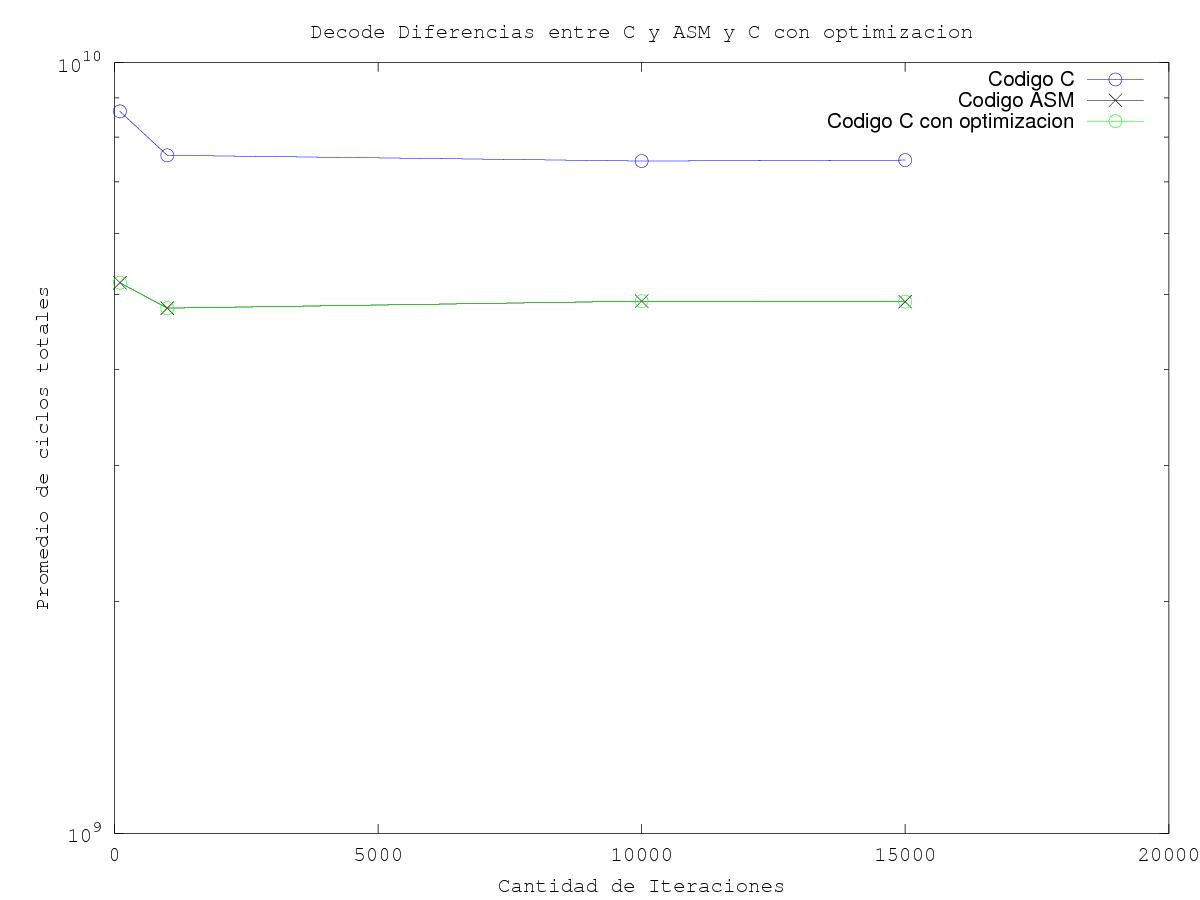
\includegraphics[scale=0.5]{imagenes/optimizacionC.jpg}
\end{center}

Esta medici\'on fue realizada cambiando la cantidad de iteraciones y midiendo cuantos ticks de procesador consume procesar el video completo. El 
problema de realizar las mediciones de esta manera es que el procesador switchea entre distintos procesos todo el tiempo haciendo que mi contador aumente
 al ejecutar procesos que no pertenecen a mi funci\'on y se cuenta en intervalos muy grandes provocando que la probabilidad de contar ticks de procesos
 exteriores sea mayor. Es por esta raz\'on que nuestra medici\'on no es lo suficientemente precisa. Una forma de hacerla mas precisa ser\'ia evaluando un
promedio de la cantidad de Ticks que consume por cada frame de cada iteraci\'on. Pero al trabajar en ordenes tan grandes deber\'iamos procesar demasiada
 informaci\'on que no viene al caso de lo que se queire mostrar.\newline

\end{itemize}

\vspace*{0.3cm} \noindent
\subsubsection{Experimento 4 - cpu vs. bus de memoria}

	Se desea conocer cual es el mayor limitante a la performance de este filtro en su versión ASM.

	¿Cuál es el factor que limita la performance en este caso? En caso de que el limitante
	fuera la intensidad de cómputo, entonces podrían agregarse instrucciones que realicen
	accesos a memoria y la performance casi no debería sufrir. La inversa puede aplicarse
	si el limitante es la cantidad de accesos a memoria.
	
	Realizar un experimento, agregando múltiples instrucciones de un mismo tipo y realizar un análisis
	del resultado. Acompañar con un gráfico.
\vspace*{0.3cm} \noindent

Nuestro algoritmo de Tiles, en su versión ASM, lo que hace es simple:\vspace*{0.3cm} \noindent

Hace unos pequeños cálculos para localizar la parte de la matriz fuente a copiar en la 
matriz destino. Luego lo que hace sencillamente es copiar a secas esa submatriz de la 
matriz destino en la matriz a devolver, esto lo hace repetidas veces. 
Entonces nuestro algoritmo hace muy pocas instrucciones de procesamiento (desempaquetar, 
dividir, aplicar máscaras, etcétera) y accede muchas veces a memoria, lo que nos hace pensar 
que el limitante de nuestro algoritmo es acceder tanto a memoria.\vspace*{0.3cm} \noindent

Para tratar de probar o negar esto, modificamos el código agregando varias instrucciones de 
procesamiento dentro del ciclo principal del algoritmo y comparamos su eficiencia en cuanto a 
tiempo con respecto al original.\vspace*{0.3cm} \noindent

Lo que vamos a hacer es agregarle al código, en su ciclo principal, las siguientes operaciones 
de procesamiento:\vspace*{0.3cm} \noindent


MOVDQU XMM1, XMM0

PXOR XMM7, XMM7 

PUNPCKLBW XMM0, XMM7

PUNPCKHBW XMM1, XMM7

PACKUSWB XMM0, XMM1
\vspace*{0.3cm} \noindent

Estas instrucciones las ponemos justo después de levantar los píxeles en xmm0, no modifican en 
nada el resultado del algoritmo.\vspace*{0.3cm} \noindent

\begin{center}
 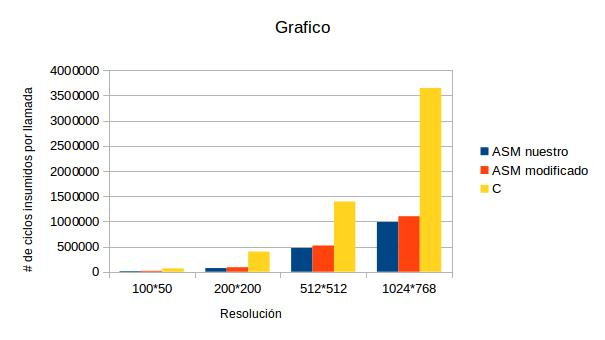
\includegraphics[scale=0.7]{tilesmod.jpg}
\end{center}

En el gráfico tenemos el tiles de ASM modificado y lo comparamos con el tiles nuestro y con el tiles de C.\vspace*{0.3cm} \noindent

Podemos ver que la cantidad de ciclos insumidos por llamada del algoritmo modificado, aunque aumentan, 
este aumento no es demasiado (nunca aumenta más de un 15\%) con respecto a nuestro ASM, y mucho menos se 
nota si lo comparamos con los valores del algoritmo hecho en C. \vspace*{0.3cm} \noindent

Esto nos deja en claro que el limitante de nuestro algoritmo son los accesos a memoria, ya que no realiza 
casi ninguna instrucción de prosesamiento en el ciclo principal del algoritmo \vspace*{0.3cm} \noindent


\newpage

\subsection{Filtro Popart}

\vspace*{0.3cm} \noindent
\subsubsection{Desarrollo Implementacion C}

En esta implementación, inicialmente,se crearon dos punteros de matriz uno correspondiente a src y otro a dst.\newline 
Ademas, un entero llamado $suma$ inicializado en 0. \newline
Luego, realizamos dos ciclos, uno añidado dentro del otro recorriendo de la forma $'(int\ i\_d = 0;\ i\_d < filas;\ i\_d++)'$ y 
$(int\ j\_d = 0;\ j\_d < cols;\ j\_d++)$.\newline
Dentro del segundo ciclo, creamos dos punteros rgb\_t donde uno apuntará a \newline rgb\_t $*p\_d = (rgb\_t*)\  \&dst\_matrix[i\_d][j\_d*3]$, y el otro
a $rgb\_t *p\_s = (rgb\_t*)\ \&src\_matrix[i\_d][j\_d]$.\newline
Al entero $suma$ le guardamos la suma de los correspondientes r, g y b del puntero p\_s $suma = p\_s\rightarrow r + p\_s\rightarrow b + p\_s\rightarrow g$ \newline
Posteriormente, chequeamos el valor correspondiente de suma:\newline Primero si $suma < 153$, en caso verdadero, guardamos en el puntero p\_d la posicion 0 de la matriz colores
$*p\_d = colores[0]$. \newline Segundo, si $(153 <= suma \  \&\& \ suma < 306)$, en caso verdadero, guardamos en el puntero p\_d la posicion 1 de la matriz colores
$*p\_d = colores[1]$.\newline Tercero, si $(306 <= suma \  \&\& \  suma < 459)$, en caso verdadero, guardamos en el puntero p\_d la posicion 2 de la matriz colores
$*p\_d = colores[2]$.\newline Cuarto, si $(459 <= suma \  \&\& \  suma < 612)$, en caso verdadero, guardamos en el puntero p\_d la posicion 3 de la matriz colores
$*p\_d = colores[3]$.\newline Por ultimo, si $(612 <= suma)$, en caso verdadero, guardamos en el puntero p\_d la posicion 4 de la matriz colores
$*p\_d = colores[4]$.\newline
Esta matriz colores mencionada se encuentra definida fuera de la funcion como:\newline \noindent
rgb\_t colores[] =  \{ \{255,   0,   0\},\newline
    \hspace*{2.8cm}  \{127,   0, 127\}\,\newline
    \hspace*{2.8cm}               $\{255,   0, 255\}\,$\newline
     \hspace*{2.8cm}              $\{  0,   0, 255\}\,$\newline
	\hspace*{2.8cm}	     $\{  0, 255, 255\} \}\;$
\vspace*{0.3cm} \noindent\newline
Estos dos ciclos realizaran $j\_d = cols - 1$  por $i\_d = filas -1$ de itereaciones.\newline
Con lo mencionado, obtenemos el filtro popart en c correctamente, con los valores que nos pasan como parámetros.\newline

\vspace*{0.3cm} \noindent
\subsubsection{Desarrollo Implementacion en ASM}
En esta implementacion, inicialmente pusheamos RBP, R12 y R13, nos guardamos en R12 y R13 los respectivos valores de columnas y filas.\newline
Luego, guardamos en EAX un 3, guardamos en R10D, R13D y procedemos a hacer la operacion MUL R10, luego realizamos lo mismo con R12 y así,
obtenemos en R10 el valor completo de la cantidad de pixeles a recorrer.\newline
Guardamos en R11 el valor de RDI donde venia *src y en R13 el valor de RSI donde venia *dst. \newline
Luego, realizamos la seccion donde chequeamos si estamos en el final de la linea o mejor dicho en el padding, comparamos con R10D si es cero \newline
en caso de ser 0 significa que ya recorrimos toda la imagen completa por ende saltamos a la etiqueta fin. \newline
En caso de no ser cero, comparamos r15d con 15, en r15 teníamos guardado la cantidad de pixel que vamos a recorrer en una iteracion.
Como vemos de a 15 pixeles si el valor es menor significa que estamos por tocar el padding y eso lo chequeamos a parte. \newline
Si no es menor, procedemos a recorrer y trabajar con 15 pixeles de la siguiente forma: \newline
Primero, nos guardamos en XMM0 los primeros 15 pixeles haciendo $ movdqu\  XMM0, [RDI]$, luego, el valor de XMM0,
lo guardamos en XMM1 y XMM2, limpiamos XMM7 y con 3 mascaras distintas que lo que hacen es ponernos los 5 pixeles rojos adelante y llenar con 0, 
los 5 pixeles azules y llenar con cero y los 5 pixeles verdes y llenar con ceros. \newline
Realizamos la operacion Pshufb con los tres xmm y las mascaras (un xmm con cada mascara) y luego desempaquetamos de byte a word,
usando el xmm7 que habiamos llenado de 0. \newline
El desempaquetado hace que nos queden los valores en word en los registros XMM10, XMM12, XMM14 respectivamente, y luego
los sumamos con PADDW guardando el valor en XMM10. De esta forma obtenemos en word 
$|b0 + g0 + r0|b1 + g1 + r1|b2 + g2 + r2|b3 + g3 + r3|b4 + g4 + r4|$. \newline
Limpiamos todos los registros que usamos, salvo XMM10 y volvemos a guardar en XMM0 el valor de XMM10 procedemos a las comparaciones.
Primero, vamos a comparar si nuestras sumas son mayores a 611, guardamos en XMM14 el valor 611 con una mascara en DW la cual tiene en todos los pack
el 611. Guardamos en XMM15 el valor XMM0 y comparamos con XMM14.
A partir del resultado en XMM15 realizamos lo siguiente:\newline

$\hspace*{2.3cm}$$movdqu\ XMM13, [MASK\_5] $\newline$ 
$\hspace*{2.8cm}$PADDUSW\ XMM10,\ XMM15 $\newline$
$\hspace*{2.8cm}$movdqu\ XMM11,\ XMM15$\newline$
$\hspace*{2.8cm}$pcmpeqw\ XMM14,\ XMM14$\newline$
$\hspace*{2.8cm}$pxor\ XMM11,\ XMM14$\newline$
$\hspace*{2.8cm}$pand\ XMM0,\ XMM11$\newline$
$\hspace*{2.8cm}$pshufb\ XMM15, [MASK\_DE1WORDA3BYTES]$\newline$
$\hspace*{2.8cm}$pand\ XMM13,\ XMM15$\newline$
$\hspace*{2.8cm}$movdqu\ XMM5,\ XMM13$ \newline

En MASK\_5 tenemos en DW los pack de los resultados que da el caso 5 osea $0|FF|FF$. Luego, en\ XMM10 lo usamos para saturar en 1 los casos que ya 
son chequeados para así no pisarlos con los otros casos. \newline
Lo salvamos y lo invertimos osea de 00 a FF y viceversa y luego hacemos un AND con los pack de\ XMM0 para quedarnos con los valores que no dieron TRUE. \newline
Usamos una mascara para que nos acomode todo de 1word a 3 bytes, hacemos otro AND con los valores TRUE y lo guardamos en\ XMM5. \newline

Despues de chequear este caso pasamos al caso 4: \newline

Primero, vamos a comparar si nuestras sumas son mayores a 458, guardamos en XMM14 el valor 458 con una mascara en DW la cual tiene en todos los pack
el 458. Guardamos en XMM15 el valor XMM0 y comparamos con XMM14.
A partir del resultado en XMM15 realizamos lo siguiente:

$\hspace*{2.3cm}$$movdqu\ XMM13, [MASK\_4] $\newline$
$\hspace*{2.8cm}$PADDUSW\ XMM10,\ XMM15 $\newline$
$\hspace*{2.8cm}$movdqu\ XMM11,\ XMM15$\newline$
$\hspace*{2.8cm}$pcmpeqw\ XMM14,\ XMM14$\newline$
$\hspace*{2.8cm}$pxor\ XMM11,\ XMM14$\newline$
$\hspace*{2.8cm}$pand\ XMM0,\ XMM11$\newline$
$\hspace*{2.8cm}$pshufb\ XMM15, [MASK\_DE1WORDA3BYTES]$\newline$
$\hspace*{2.8cm}$pand\ XMM13,\ XMM15$\newline$
$\hspace*{2.8cm}$movdqu\ XMM4,\ XMM13$ \newline

En MASK\_4 tenemos en DW los pack de los resultados que da el caso 4 osea $0|0|FF$. Luego, en XMM10 lo usamos para saturar en 1 los casos que ya 
son chequeados para así no pisarlos con los otros casos. \newline
Lo salvamos y lo invertimos osea de 00 a FF y viceversa y luego hacemos un AND con los pack de XMM0 para quedarnos con los valores que no dieron TRUE. \newline
Usamos una mascara para que nos acomode todo de 1word a 3 bytes, hacemos otro AND con los valores TRUE y lo guardamos en XMM4. \newline

Despues de chequear este caso pasamos al caso 3: \newline

Primero, vamos a comparar si nuestras sumas son mayores a 305, guardamos en XMM14 el valor 305 con una mascara en DW la cual tiene en todos los pack
el 305. Guardamos en XMM15 el valor XMM0 y comparamos con XMM14.
A partir del resultado en XMM15 realizamos lo siguiente:\newline

$\hspace*{2.3cm}$$movdqu\ XMM13, [MASK\_3] $\newline$
$\hspace*{2.8cm}$PADDUSW\ XMM10,\ XMM15 $\newline$
$\hspace*{2.8cm}$movdqu\ XMM11,\ XMM15$\newline$
$\hspace*{2.8cm}$pcmpeqw\ XMM14,\ XMM14$\newline$
$\hspace*{2.8cm}$pxor\ XMM11,\ XMM14$\newline$
$\hspace*{2.8cm}$pand\ XMM0,\ XMM11$\newline$
$\hspace*{2.8cm}$pshufb\ XMM15, [MASK\_DE1WORDA3BYTES]$\newline$
$\hspace*{2.8cm}$pand\ XMM13,\ XMM15$\newline$
$\hspace*{2.8cm}$movdqu\ XMM3,\ XMM13$ \newline

En MASK\_3 tenemos en DW los pack de los resultados que da el caso 3 osea $FF|0|FF$. Luego, en XMM10 lo usamos para saturar en 1 los casos que ya 
son chequeados para así no pisarlos con los otros casos. \newline
Lo salvamos y lo invertimos osea de 00 a FF y viceversa y luego hacemos un AND con los pack de XMM0 para quedarnos con los valores que no dieron TRUE. \newline
Usamos una mascara para que nos acomode todo de 1word a 3 bytes, hacemos otro AND con los valores TRUE y lo guardamos en XMM3. \newline

Despues de chequear este caso pasamos al caso 2: \newline

Primero, vamos a comparar si nuestras sumas son mayores a 152, guardamos en XMM14 el valor 152 con una mascara en DW la cual tiene en todos los pack
el 152. Guardamos en XMM15 el valor XMM0 y comparamos con XMM14.
A partir del resultado en XMM15 realizamos lo siguiente:

$\hspace*{2.3cm}$$movdqu\ XMM13, [MASK\_2] $\newline$
$\hspace*{2.8cm}$PADDUSW\ XMM10,\ XMM15 $\newline$
$\hspace*{2.8cm}$movdqu\ XMM11,\ XMM15$\newline$
$\hspace*{2.8cm}$pcmpeqw\ XMM14,\ XMM14$\newline$
$\hspace*{2.8cm}$pxor\ XMM11,\ XMM14$\newline$
$\hspace*{2.8cm}$pand\ XMM0,\ XMM11$\newline$
$\hspace*{2.8cm}$pshufb\ XMM15, [MASK\_DE1WORDA3BYTES]$\newline$
$\hspace*{2.8cm}$pand\ XMM13,\ XMM15$\newline$
$\hspace*{2.8cm}$movdqu\ XMM2,\ XMM13$ \newline

En MASK\_2 tenemos en DW los pack de los resultados que da el caso 2 osea $7F|0|7F$. Luego, en XMM10 lo usamos para saturar en 1 los casos que ya 
son chequeados para así no pisarlos con los otros casos. \newline
Lo salvamos y lo invertimos osea de 00 a FF y viceversa y luego hacemos un AND con los pack de XMM0 para quedarnos con los valores que no dieron TRUE. \newline
Usamos una mascara para que nos acomode todo de 1word a 3 bytes, hacemos otro AND con los valores TRUE y lo guardamos en XMM2. \newline

Y por último, el caso 1:\newline

Este caso, es particular, ya que invertimos, y chequeamos si los packs que quedan son menores a 153: \newline

$\hspace*{2.3cm}$$movdqa\ XMM14,[MASK\_153]$\newline$
$\hspace*{2.8cm}$			movdqu\ XMM6,\ XMM10 ; me quedo con\ XMM10 y trabajamos  el de\ XMM6$\newline$
$\hspace*{2.8cm}$			pcmpeqw\ XMM7,\ XMM7 ;\ XMM7 = |1|1|1|1|1|1|1|1|1|1|1|1|1|1|1|1$\newline$
$\hspace*{2.8cm}$			pxor\ XMM6,\ XMM7 ; deja en 1 este caso y 0 los casos ya checkeados$\newline$
$\hspace*{2.8cm}$			pand\ XMM14,\ XMM6 ; en\ XMM14 queda los 153 en los lugares que tengo que comparar$\newline$
$\hspace*{2.8cm}$			movdqu\ XMM15,\ XMM0$\newline$
$\hspace*{2.8cm}$			pcmpgtw\ XMM14,\ XMM15 $$\newline$

			A partir del resultado en XMM14 realizamos lo siguiente:\newline

$\hspace*{2.3cm}$$movdqu\ XMM13, [MASK\_1] $\newline$
$\hspace*{2.8cm}$PADDUSW\ XMM10,\ XMM14 $\newline$
$\hspace*{2.8cm}$movdqu\ XMM11,\ XMM14$\newline$
$\hspace*{2.8cm}$pcmpeqw\ XMM15,\ XMM15$\newline$
$\hspace*{2.8cm}$pxor\ XMM11,\ XMM15$\newline$
$\hspace*{2.8cm}$pand\ XMM0,\ XMM11$\newline$
$\hspace*{2.8cm}$pshufb\ XMM14, [MASK\_DE1WORDA3BYTES]$\newline$
$\hspace*{2.8cm}$pand\ XMM13,\ XMM14$\newline$
$\hspace*{2.8cm}$movdqu\ XMM1,\ XMM13$ \newline

En MASK\_1 tenemos en DW los pack de los resultados que da el caso 1 osea $FF|0|0$. Luego, en XMM10 lo usamos para saturar en 1 los casos que ya 
son chequeados para así no pisarlos con los otros casos. \newline
Lo salvamos y lo invertimos osea de 00 a FF y viceversa y luego hacemos un AND con los pack de XMM0 para quedarnos con los valores que no dieron TRUE. \newline
Usamos una mascara para que nos acomode todo de 1word a 3 bytes, hacemos otro AND con los valores TRUE y lo guardamos en XMM1. \newline

Por finalizado, hacemos or entre los XMM1, 2, 3, 4 y 5, y movemos el valor final de XMM1 a XMM0. \newline Comparamos si estamos 
chequeando el borde haciendo $ cmp\  r15d, 15 jl .terminoBorde $ en caso de no ser menor movemos los packs del XMM0 al puntero
en RDI $movdqu\  [RSI], XMM0$, le restamos a r15d y a r10d, la cantidad de pixeles por ciclo y le sumamos a rdi y rsi la cantidad
de pixeles por ciclo. \newline

En caso de que nuestra comparacion diera que es menor a 15, procedemos a: \newline

$\hspace*{2.3cm}$$movdqu [RSI- pixels\_por\_ciclo + r12],\ XMM0 $\newline$
$\hspace*{2.8cm}$		add r11, r8 $\newline$
$\hspace*{2.8cm}$		add r13, r8 $\newline$
$\hspace*{2.8cm}$		mov RDI, r11 $\newline$
$\hspace*{2.8cm}$		mov r11, rdi  $\newline$
$\hspace*{2.8cm}$		mov RSI, r13 $\newline$
$\hspace*{2.8cm}$		mov r13, rsi $\newline$
$\hspace*{2.8cm}$		sub R10D, r15d $\newline$
$\hspace*{2.8cm}$		mov r15d, r14d$ \newline

Como habiamos enuciado inicialmente, en R11 y R13 nos habiamos guardado RDI y RSI respectivamente y en R8 tenemos por parametro
$src\_row\_size$. De esta forma hacemos que en dst se guarden los ultimos pixeles de la linea y baje a la siguiente sin tocar padding.\newline

Esto, como fue explicado, se recorre, hasta que R10D sea igual a 0.


\vspace*{0.3cm} \noindent
\subsubsection{Experimento 1 - saltos condicionales}

	Se desea conocer que tanto impactan los saltos condicionales
	en el código del ejercicio anterior con \verb|-O1|.\\
	Para poder medir esto, una posibilidad es quitar las comparaciones
	al procesar cada pixel. Por más que la imagen resultante no sea correcta,
	será posible tomar una medida del impacto de los saltos condicionales.
	Analizar como varía la performance. 
	
	Si se le ocurren, mencionar otras posibles formas de medir el impacto de los saltos condicionales.
	
	
  \vspace*{0.3cm} 


 Para poder conocer como impactaban los saltos condicionales en la implementacion realizamos distintas mediciones;
 quitando los saltos con y sin optimizacion obteniendo los siguientes resultados:
 Quitando los saltos sin optimizar obtuvimos que, para imagenes de tamaño pequeño (50x100) con 100 iteraciones, el mencionado codigo insume
 una cantidad de 389596 ciclos por cada llamada. A su vez, con imagenes de tamaño mas grande (200x200) utilizando la misma cantidad de iteraciones,
 el codigo nos insume  una cantidad de 1803084 ciclos por llamada, mientras que con imagenes aun mas grande como por ejemplo 512x512 y 1024x768, demanda
 10745530 y 32020980 por llamada respectivamente.
 \vspace*{0.3cm} 
 Mientras que la implementación sin saltos con optimizacion -O1 cosechamos la siguiente información:
 Para imagenes de tamaño pequeño (50x100) con la misma cantidad de iteraciones insume 167132 ciclos por llamada. 
 Con imagenes de mayor tamaño (200x200), demanda 805378 de ciclos.
 Por ultimo con imagenes de tamaño aun mayor (512x512) y (1024x768), emplea 4719143 y 13811050 de ciclos por llamada correspondientemente.
  \vspace*{0.3cm}
 
  Para una mejor representación se realizo un grafico mostrando a simple vista
  las diferencias entre cada tipo de version de la implementacion implementacion.
 \vspace*{0.3cm} \vspace*{0.3cm}
  \begin{center}
 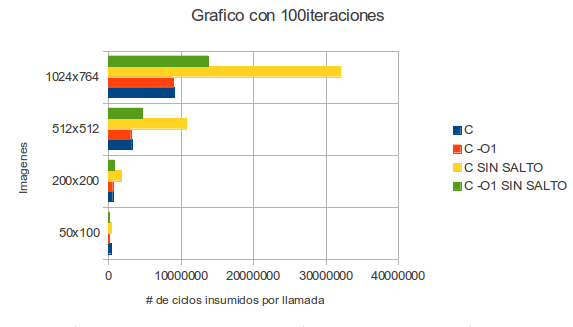
\includegraphics[scale=0.7]{popartbien.png}
 \end{center}
  \vspace*{0.3cm} 

  Concluimos que en imagenes grandes es muy notoria la diferencia en performace entre las versiones con y sin saltos.

\vspace*{0.3cm} \noindent
\subsubsection{Experimento 2 - cpu vs. bus de memoria}

	¿Cuál es el factor que limita la performance en este caso? 
	
	Realizar un experimento, agregando múltiples instrucciones de un mismo tipo
	y realizar un análisis 	del resultado. Acompañar con un gráfico.\vspace*{0.3cm} \noindent

  



  En este caso lo que limita a la performance son las comparaciones y saltos condicionales.
  Para probar esto agregamos instrucciones de varios tipos en la versión de ASM: accesos a memoria, 
  movimiento de registros, sumas, comparaciones y finalmente comparaciones y saltos. \vspace*{0.2cm} \noindent




  Todas estas agregadas en cada instacia de procesamiento, es decir, tomamos el dato, lo procesamos,
  agregamos las instrucciones (50) y así sucesivamente con cada dato.\vspace*{0.2cm} \noindent




  Como resultado observamos que lo que más ciclos insume son las comparaciones y saltos condicionales. 
  Este tipo de instrucciones incrementan con el tamaño de la imagen, ya que mientras mas grande es la imagen, 
  más comparaciones para fijarse si llegó al final tendrá que hacer.\vspace*{0.2cm} \noindent




  Los accesos a memoria también son costosos, pero quedaron en segundo lugar.\vspace*{0.2cm} \noindent
  
  A continuación enunciaremos los respectivos ciclos insumidos por llamada dependiendo cada caso y cada 
  resolución de imagen.\vspace*{0.3cm} \noindent
 
 120x56 
 
+50 accesos		: 124262.398

+50 movimientos		: 85166.438

+50 sumas		: 100156.117

+50 comparaciones	: 106732.922

+50 comp y saltos	: 233104.562

\vspace*{0.3cm} \noindent
200x200

+50 accesos		: 748478.750

+50 movimientos		: 511008.031

+50 sumas		: 584339.938

+50 comparaciones	: 578177.250

+50 comp y saltos	: 1411856.125

\vspace*{0.3cm} \noindent
512x512

+50 accesos		: 5279703.500

+50 movimientos		: 3266983.000

+50 sumas		: 3802452.750

+50 comparaciones	: 4524299.000

+50 comp y saltos	: 9041962.000

\vspace*{0.3cm} \noindent
1023x767

+50 accesos		: 18832506.000

+50 movimientos		: 12843421.000

+50 sumas		: 15499867.000

+50 comparaciones	: 15349734.000

+50 comp y saltos	: 28297848.000

\vspace*{0.3cm} \noindent

  En el siguiente gráfico podemos distinguir los resultados.
  \vspace*{0.2cm} \noindent\vspace*{0.2cm} \noindent


  \begin{center}
 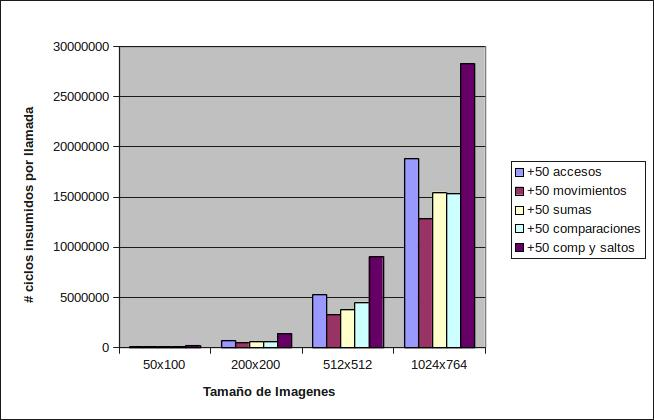
\includegraphics[scale=0.7]{popart2.jpg}
 \end{center}
  \vspace*{0.3cm} 
  


\vspace*{0.3cm} \noindent
\subsubsection{Experimento 3 - prefetch}

  La técnica de \textit{prefetch} es otra forma de optimización que puede
  realizarse. Su sustento teórico es el siguiente:
  
  Suponga un algoritmo que en cada iteración tarda n ciclos en obtener un dato y una cantidad
  similar en procesarlo. Si el algoritmo lee el dato $i$ y luego lo procesa,
  desperdiciará siempre n ciclos esperando entre que el dato llega y que se comienza
  a procesar efectivamente. Un algoritmo más inteligente podría pedir el 
  dato $i+1$ al comienzo del ciclo de proceso del dato $i$ (siempre suponiendo
  que el dato $i$ pidió en la iteración $i-1$. De esta manera, a la vez que el
  procesador computa todas las instrucciones de la iteración $i$, se estáran trayendo
  los datos de la siguiente iteración, y cuando esta última comience, los datos ya
  habrán llegado.  \vspace*{0.2cm}

  

  Estudiar esta técnica y proponer una aplicación al código del filtro en la versión ASM.
  Programarla y analizar el resultado. ¿Vale la pena hacer prefetching?\vspace*{0.2cm}
  
  
  
  
  Cuando empezamos a estudiar esta técnica, creímos que no era realizable en assembler, 
  ya que pensamos que cada instrucción era bloqueante, es decir, 
  que hasta que no se terminaba de ejecutar una instrucción no seguía con la siguiente. \vspace*{0.2cm}
 
 
 
  Luego descubrimos que no era así. El procesador puede ejecutar las instrucciones fuera de orden. 
  Si no es necesario, o no depende de la instrucción anterior, el procesador no espera a que se 
  termine de ejecutar la instrucción actual para ejecutar la siguiente.\vspace*{0.2cm}



  Para probar esto, adaptamos el prefecth a assembler. Modificamos levemente el recorrido de la 
  imagen para no hacer accesos a memoria, al menos no directamente. Lo hicimos a través de un registro.
  Por ejemplo, levantamos de memoria en XMM8, luego lo pasamos a XMM0 y seguimos levantando de memoria 
  la siguiente posición en XMM8. Así mientras se procesa el dato de XMM0 se puede ir trayendo el 
  siguiente dato a procesar en XMM8.\vspace*{0.2cm}
  
  A continuación, enunciaremos los valores obtenidos de nuestras mediciones en las respectivas resoluciones
  utilizando prefecth y sin utilizarlo.\vspace*{0.3cm} \noindent
  
  \vspace*{0.3cm} \noindent
  \vspace*{0.3cm} \noindent
120x56

\vspace*{0.1cm} \noindent

sin prefetch: 67836.359

con prefetch: 65300.320

\vspace*{0.3cm} \noindent
200x200
\vspace*{0.1cm} \noindent

sin prefetch: 398975.594

con prefetch: 382423.562

\vspace*{0.3cm} \noindent
512x512

\vspace*{0.1cm} \noindent

sin prefetch: 2498557.750

con prefetch: 2438276.250

\vspace*{0.3cm} \noindent
1023x767

\vspace*{0.1cm} \noindent

sin prefetch: 10389265.000

con prefetch: 7434984.500

\vspace*{0.3cm} \noindent

 \begin{center}
 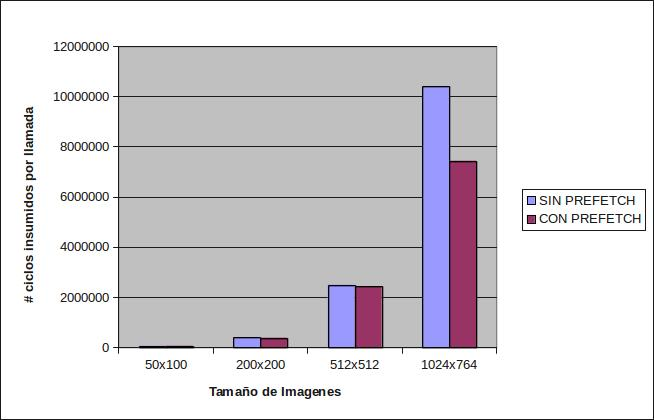
\includegraphics[scale=0.7]{popart3.jpg}
 \end{center}
  \vspace*{0.3cm} 
  
  Se puede observar que hay una sutil mejora en la performance en tamaños pequeños y medianos. 
  En cambio en la imagen grande, se puede observar una brecha más amplia.\vspace*{0.2cm}



  Lógicamente, mientras más grande es la imagen, la mejora será más notoria al haber más accesos a memoria.\vspace*{0.2cm}




  Como conclusión decimos que no vale la pena hacer prefetching para este filtro,
  ya que la diferencia se puede apreciar sólo en imágenes grandes, y además te restringe el uso de un registro XMM.

\vspace*{0.3cm} \noindent
\subsubsection{Experimento 4 - secuencial vs. vectorial}

  Analizar cuales son las diferencias de performace entre las versiones de C y ASM. 
  Realizar gráficos que representen estas diferencias.

  
 Realizando nuestras mediciones en la implementacion de C y en ASM obtenemos los siguientes resultados:\vspace*{0.3cm} \noindent
 
\vspace*{0.3cm} \noindent
120x56

En ASM: 444959

En C: 128763


\vspace*{0.3cm} \noindent
200x200

En ASM: 631827

En C: 628630


\vspace*{0.3cm} \noindent
512x512

En ASM: 3261260

En C: 3098234


\vspace*{0.3cm} \noindent
1023x767

En ASM: 9107332

En C: 8978195


\vspace*{0.3cm}

 Para una mejor representación se realizaron distintos graficos mostrando a simple vista
 las diferencias entre cada tipo de implementacion en cada tipo de imagen.
 \vspace*{0.3cm} \vspace*{0.3cm}
  \begin{center}
 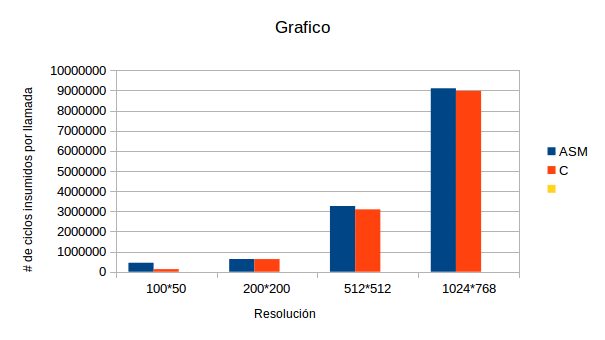
\includegraphics[scale=0.8]{asmc.png}
 \end{center}
  \vspace*{0.3cm} 
  
  La diferencia principal entre el c\'odigo escrito en lenguaje C y el c\'odigo ASM, es la cantidad de accesos 
a memoria realizados en cada iteraci\'on. Otra diferencia puede verse en la cantidad de bytes que pueden 
ser procesados simultaneamente durante el mismo ciclo. 
Mientras que en C leemos y procesamos un byte por vez, el c\'odigo ASM nos permite acceder y procesar 
16 bytes en simultaneos. De todas maneras, en este caso trabajamos con 12 bytes que es un numero mas \'util 
ya que es m\'ultiplo de 3 (cantidad de bytes por p\'ixel)  y de 4 (cantidad de bytes por cada caracter).
Pudiendo levantar de a 16 bytes en memoria, podr\'ia esperarse que el c\'odigo asm demorase una 
diesiseiava parte de la cantidad de ciclos que demora el c\'odigo en C.
Pero debemos tener en cuenta que en nuestro caso estamos aprovechando solo 15 de los 16 bytes que leemos 
en cada iteraci\'on por lo tanto es más acertado evaluar como si solo leyeramos 15 bytes. 
Adem\'as, hay que tener en cuenta que las instrucciones SSE pueden necesitar más ciclos que las operaciones 
comunes que usamos en el C, eso disminuye un poco la performance en la comparación. 
Por mas que como hemos visto los saltos condicionales empeoran la performace en ASM, dicha implementacion
sigue siendo mas optima que la de C.
\vspace*{0.3cm} \vspace*{0.3cm} 

\newpage
\subsection{Filtro Temperature}

\vspace*{0.3cm} \noindent
\subsubsection{Desarrollo Implementacion C}

En esta implementación, inicialmente,se crearon dos punteros de matriz uno correspondiente a src y otro a dst.\newline 
Ademas, un entero llamado $suma$ y otro $divido$ inicializados en 0. \newline
Luego, realizamos dos ciclos, uno añidado dentro del otro recorriendo de la forma $'(int\ i\_d = 0;\ i\_d < filas;\ i\_d++)'$ y 
$(int\ j\_d = 0;\ j\_d < cols;\ j\_d++)$.\newline
Dentro del segundo ciclo, creamos dos punteros rgb\_t donde uno apuntará a \newline rgb\_t $*p\_d = (rgb\_t*)\  \&dst\_matrix[i\_d][j\_d*3]$, y el otro
a $rgb\_t *p\_s = (rgb\_t*)\ \&src\_matrix[i\_d][j\_d]$.\newline
Al entero $suma$ le guardamos la suma de los correspondientes r, g y b del puntero p\_s $suma = p\_s\rightarrow r + p\_s\rightarrow b + p\_s\rightarrow g$
Al entero $divido$ le guardamos el valor de suma dividido por 3 $ divido = suma/3$
Posteriormente, chequeamos entre que valores se encuentra divido utilizando la funcion between provista por la catedra:\vspace*{0.3cm} \noindent\newline 
Primero si $(between(divido,0,31))$, en caso verdadero, guardamos en el valor r del puntero p\_d el valor 0,en el valor g 
guardamos el valor 0 y en el valor b guardamos $(128+ (4*divido)$. \newline 
Segundo, si $(between(divido,32,95))$, en caso verdadero, guardamos en el valor r del puntero p\_d el valor 0,en el valor g 
guardamos el valor $(divido-32)*4$ y en el valor b guardamos 255. \newline Tercero, si $(between(divido,96,159))$, en caso verdadero, guardamos en el valor r del puntero p\_d el valor $(divido-96)*4$,en el valor g 
guardamos el valor 255 y en el valor b guardamos $255-((divido-96)*4)$. \newline Cuarto, si $(between(divido,160,223))$, en caso verdadero, guardamos en el valor r del puntero p\_d el valor 255,en el valor g 
guardamos el valor $255 - ((divido-160)*4)$ y en el valor b guardamos 0. \newline  Por ultimo, si $(between(divido,224,255))$, en caso verdadero, guardamos en el valor r del puntero p\_d el valor $255-(divido-224)*4$,en el valor g 
guardamos el valor 0 y en el valor b guardamos 0. \newline 

Estos dos ciclos realizaran $j\_d = cols - 1$  por $i\_d = filas -1$ de itereaciones.\newline
Con lo mencionado, obtenemos el filtro temperature en c correctamente, con los valores que nos pasan como parámetros.\newline

\vspace*{0.3cm} \noindent
\subsubsection{Desarrollo Implementacion en ASM}
En esta implementacion, inicialmente pusheamos RBP, R12 y R13, nos guardamos en R12 y R13 los respectivos valores de columnas y filas.\newline
Luego, guardamos en EAX un 3, guardamos en R10D, R13D y procedemos a hacer la operacion MUL R10, luego realizamos lo mismo con R12 y así,
obtenemos en R10 el valor completo de la cantidad de pixeles a recorrer.\newline
Guardamos en R11 el valor de RDI donde venia *src y en R13 el valor de RSI donde venia *dst. \newline
Luego, realizamos la seccion donde chequeamos si estamos en el final de la linea o mejor dicho en el padding, comparamos con R10D si es cero \newline
en caso de ser 0 significa que ya recorrimos toda la imagen completa por ende saltamos a la etiqueta fin. \newline
En caso de no ser cero, comparamos r15d con 15, en r15 teníamos guardado la cantidad de pixel que vamos a recorrer en una iteracion.
Como vemos de a 15 pixeles si el valor es menor significa que estamos por tocar el padding y eso lo chequeamos a parte. \newline
Si no es menor, procedemos a recorrer y trabajar con 15 pixeles de la siguiente forma: \newline
Primero, nos guardamos en XMM0 los primeros 15 pixeles haciendo $ movdqu\  XMM0, [RDI]$, luego, el valor de XMM0,
lo guardamos en XMM1 y XMM2, limpiamos XMM7 y con 3 mascaras distintas que lo que hacen es ponernos los 5 pixeles rojos adelante y llenar con 0, 
los 5 pixeles azules y llenar con cero y los 5 pixeles verdes y llenar con ceros. \newline
Realizamos la operacion Pshufb con los tres xmm y las mascaras (un xmm con cada mascara) y luego desempaquetamos de byte a word,
usando el xmm7 que habiamos llenado de 0. \newline
El desempaquetado hace que nos queden los valores en word en los registros XMM10, XMM12, XMM14 respectivamente, y luego
los sumamos con PADDW guardando el valor en XMM10. De esta forma obtenemos en word 
$|b0 + g0 + r0|b1 + g1 + r1|b2 + g2 + r2|b3 + g3 + r3|b4 + g4 + r4|$. \newline
Limpiamos todos los registros que usamos, salvo XMM10 y volvemos a guardar en XMM0 el valor de XMM10. Luego, procedemos
a realizar la division correspondiente de los packs de la siguiente manera:\newline

$movdqu xmm10, [DIVIDO]$\newline$
$\hspace*{2.3cm}$	movdqu xmm1, xmm0$\newline$
$\hspace*{2.8cm}$		movdqu xmm2, xmm0$\newline$
		$\hspace*{2.8cm}$XORPD xmm15, xmm15$\newline$
		$\hspace*{2.8cm}$punpcklwd xmm1, xmm15$\newline$
		$\hspace*{2.8cm}$punpckhwd xmm2, xmm15$\newline$
		$\hspace*{2.8cm}$cvtdq2ps xmm1, xmm1$\newline$
		$\hspace*{2.8cm}$cvtdq2ps xmm2, xmm2$\newline$
		$\hspace*{2.8cm}$cvtdq2ps xmm10,xmm10$\newline$
		$\hspace*{2.8cm}$divps XMM1, xmm10$\newline$
		$\hspace*{2.8cm}$divps XMM2, xmm10$\newline$
		$\hspace*{2.8cm}$CVTTPS2DQ xmm1,xmm1$\newline$
		$\hspace*{2.8cm}$CVTTPS2DQ xmm2, xmm2$\newline$
		$\hspace*{2.8cm}$PACKUSDW xmm1, xmm2$\newline$
		$\hspace*{2.8cm}$movdqu xmm0, xmm1$\newline$
		 $$\newline$
	
En la mascara DIVIDO tenemos el valor 3 en DD. Desempaquetamos de Word a Dword para luego podes convertir a float.
Realizamos la respectiva division y luego volvemos a convertir de float a dword y de dword a word y volvemos a guardar
el resultado en XMM0. \newline

Limpiamos todos los registros que usamos, salvo XMM0. Posteriormente, seguimos con las comparaciones.
Primero, vamos a comparar si nuestras sumas son mayores a 223, guardamos en XMM14 el valor 223 con una mascara en DW la cual tiene en todos los pack
el 223. Guardamos en XMM15 el valor XMM0 y comparamos con XMM14.
A partir del resultado en XMM15 realizamos lo siguiente:\newline

$\hspace*{2.3cm}$$movdqu\ xmm13,\ xmm0$\newline$
		$\hspace*{2.8cm}$movdqu\ xmm11, [M224]$\newline$		
		$\hspace*{2.8cm}$psubb\ XMM13,\ xmm11$\newline$
		$\hspace*{2.8cm}$pand\ xmm13,\ xmm15$\newline$
			$\hspace*{2.8cm}$movdqu\ xmm11, [M4]$\newline$
		$\hspace*{2.8cm}$movdqu\ xmm7,\ xmm13$\newline$
		$\hspace*{2.8cm}$movdqu\ xmm8,\ xmm13$\newline$
		$\hspace*{2.8cm}$XORPD\ xmm9,\ xmm9$\newline$
		$\hspace*{2.8cm}$punpcklwd\ xmm7,\ xmm9$\newline$
		$\hspace*{2.8cm}$punpckhwd\ xmm8,\ xmm9$\newline$
		$\hspace*{2.8cm}$cvtdq2ps\ xmm7,\ xmm7$\newline$
		$\hspace*{2.8cm}$cvtdq2ps\ xmm8,\ xmm8$\newline$
		$\hspace*{2.8cm}$cvtdq2ps\ xmm11,xmm11$\newline$
		$\hspace*{2.8cm}$mulps\ XMM7,\ xmm11$\newline$
		$\hspace*{2.8cm}$mulps\ XMM8,\ xmm11$\newline$
		$\hspace*{2.8cm}$CVTPS2DQ\ xmm7,xmm7$\newline$
		$\hspace*{2.8cm}$CVTPS2DQ\ xmm8,\ xmm8$\newline$
		$\hspace*{2.8cm}$PACKUSDW\ xmm7,\ xmm8$\newline$
		$\hspace*{2.8cm}$movdqu\ xmm13,\ xmm7$\newline$
		$\hspace*{2.8cm}$movdqu\ xmm11, [M255]$\newline$
		$\hspace*{2.8cm}$pand\ xmm11,\ xmm15$\newline$
		$\hspace*{2.8cm}$psubb\ xmm11,\ xmm13$\newline$
		$\hspace*{2.8cm}$movdqu\ xmm13,\ xmm11$\newline$		
		$\hspace*{2.8cm}$pshufb\ xmm13, [MASK_5] $\newline$
		$\hspace*{2.8cm}$PADDUSW\ XMM10,\ XMM15 $\newline$
		$\hspace*{2.8cm}$movdqu\ xmm11,\ xmm15 $\newline$
		$\hspace*{2.8cm}$pcmpeqw\ XMM14,XMM14$\newline$
		$\hspace*{2.8cm}$pxor\ xmm11,\ xmm14$\newline$
		$\hspace*{2.8cm}$pand\ xmm0,xmm11$\newline$		
		$\hspace*{2.8cm}$pshufb\ XMM15, [MASK_DE1WORDA3BYTES]$\newline$
		$\hspace*{2.8cm}$pand\ xmm13,\ xmm15$\newline$
		$\hspace*{2.8cm}$movdqu\ xmm5,\ xmm13$$\newline$

Copiamos en XMM13, el valor de XMM0, guardamos en XMM11 una mascara en DW con 224, realizamos la resta de los packs y luego un and 
con XMM15 para quedarnos con los packs que cumplieron esta comparacion. Despues, guardamos en XMM11 una mascara en DW con 4.
Procedemos a desempaquetar de WORD a DWORD el XMM13 copiandolo previamente en otros dos XMM. Luego convertimos todo de DWORD
a FLOAT y realizamos la multiplicacion con XMM11. Volvemos a convertir a DWORD y a empaquetar a WORD y guardamos el resultado 
en XMM13. \newline
Guardamos en XMM11 una mascara DW con 255 realizamos un and entre este XMM y el XMM15 para quedarnos con los packs que dieron TRUE
la comparacion y luego restamos XMM11 con XMM13 y guardamos el valor de XMM11 en XMM13.
En MASK\_5 tenemos en DW los pack de los resultados que da el caso 5 osea $X|0|0$. Luego, en\ XMM10 lo usamos para saturar en 1 los casos que ya 
son chequeados para así no pisarlos con los otros casos. \newline
Lo salvamos y lo invertimos osea de 00 a FF y viceversa y luego hacemos un AND con los pack de\ XMM0 para quedarnos con los valores que no dieron TRUE. \newline
Usamos una mascara para que nos acomode todo de 1word a 3 bytes, hacemos otro AND con los valores TRUE y lo guardamos en\ XMM5. \newline

Despues de chequear este caso pasamos al caso 4: \newline

Primero, vamos a comparar si nuestras sumas son mayores a 159, guardamos en XMM14 el valor 159 con una mascara en DW la cual tiene en todos los pack
el 159. Guardamos en XMM15 el valor XMM0 y comparamos con XMM14.
A partir del resultado en XMM15 realizamos lo siguiente: \newline

$\hspace*{2.3cm}$$movdqu\ xmm13,\ xmm0$\newline$
		$\hspace*{2.8cm}$movdqu\ xmm11, [M160]$\newline$	
		$\hspace*{2.8cm}$psubb\ XMM13,\ xmm11$\newline$
		$\hspace*{2.8cm}$pand\ xmm13,\ xmm15$\newline$
		$\hspace*{2.8cm}$movdqu\ xmm11, [M4]$\newline$
		$\hspace*{2.8cm}$movdqu\ xmm7,\ xmm13$\newline$
		$\hspace*{2.8cm}$movdqu\ xmm8,\ xmm13$\newline$
		$\hspace*{2.8cm}$XORPD\ xmm9,\ xmm9$\newline$
		$\hspace*{2.8cm}$punpcklwd\ xmm7,\ xmm9$\newline$
		$\hspace*{2.8cm}$punpckhwd\ xmm8,\ xmm9$\newline$
		$\hspace*{2.8cm}$cvtdq2ps\ xmm7,\ xmm7$\newline$
		$\hspace*{2.8cm}$cvtdq2ps\ xmm8,\ xmm8$\newline$
		$\hspace*{2.8cm}$cvtdq2ps\ xmm11,xmm11$\newline$
		$\hspace*{2.8cm}$mulps\ XMM7,\ xmm11$\newline$
		$\hspace*{2.8cm}$mulps\ XMM8,\ xmm11$\newline$
		$\hspace*{2.8cm}$CVTPS2DQ\ xmm7,xmm7$\newline$
		$\hspace*{2.8cm}$CVTPS2DQ\ xmm8,\ xmm8$\newline$
		$\hspace*{2.8cm}$PACKUSDW\ xmm7,\ xmm8$\newline$
		$\hspace*{2.8cm}$movdqu\ xmm13,\ xmm7
		$\newline$
		$\hspace*{2.8cm}$movdqu\ xmm11, [MASK\_4]$\newline$
		$\hspace*{2.8cm}$pshufb\ xmm13, [MASK\_4\_2]$\newline$
		$\hspace*{2.8cm}$psubb\ xmm11,\ xmm13 $\newline$
		$\hspace*{2.8cm}$movdqu\ xmm13,\ xmm11$\newline$
		$\hspace*{2.8cm}$movdqu\ xmm11,\ xmm15$\newline$
		$\hspace*{2.8cm}$pcmpeqw\ XMM14,XMM14$\newline$
		$\hspace*{2.8cm}$pxor\ xmm11,\ xmm14$\newline$
		$\hspace*{2.8cm}$pand\ xmm0,xmm11$\newline$
		$\hspace*{2.8cm}$PADDUSW\ XMM10,\ XMM15 $\newline$
		$\hspace*{2.8cm}$pshufb\ XMM15, [MASK\_DE1WORDA3BYTES]$\newline$
		$\hspace*{2.8cm}$pand\ xmm13,\ xmm15$\newline$
		$\hspace*{2.8cm}$movdqu\ xmm4,\ xmm13$$\newline$

		

Copiamos en XMM13, el valor de XMM0, guardamos en XMM11 una mascara en DW con 160, realizamos la resta de los packs y luego un and 
con XMM15 para quedarnos con los packs que cumplieron esta comparacion. Despues, guardamos en XMM11 una mascara en DW con 4.
Procedemos a desempaquetar de WORD a DWORD el XMM13 copiandolo previamente en otros dos XMM. Luego convertimos todo de DWORD
a FLOAT y realizamos la multiplicacion con XMM11. Volvemos a convertir a DWORD y a empaquetar a WORD y guardamos el resultado 
en XMM13. \newline
Guardamos en XMM11 una mascara DW con los resultados que da el caso 4 y hacemos un movimiento de Packs en XMM13 de la forma
$X|0x80|0x80$ realizamos la resta entre ambos y guardamos el resultado de XMM11 en XMM13. Guardamos en XMM11 el valor de XMM15 
invertimos el XMM11 y luego hacemos un and con XMM0.\newline
Luego, en\ XMM10 lo usamos para saturar en 1 los casos que ya son chequeados para así no pisarlos con los otros casos. \newline
Usamos una mascara para que nos acomode todo de 1word a 3 bytes, hacemos otro AND con los valores TRUE y lo guardamos en\ XMM4. \newline

Despues de chequear este caso pasamos al caso 3: \newline

Primero, vamos a comparar si nuestras sumas son mayores a 95, guardamos en\ XMM14 el valor 95 con una mascara en DW la cual tiene en todos los pack
el 95. Guardamos en\ XMM15 el valor\ XMM0 y comparamos con\ XMM14.
A partir del resultado en\ XMM15 realizamos lo siguiente:\newline

	$\hspace*{2.3cm}$$movdqu\ xmm13,\ xmm0$\newline$
		$\hspace*{2.8cm}$movdqu\ xmm11, [M96]$\newline$	
		$\hspace*{2.8cm}$psubb\ XMM13,\ XMM11$\newline$
		$\hspace*{2.8cm}$pand\ xmm13,\ xmm15$\newline$
		$\hspace*{2.8cm}$movdqu\ xmm11, [M4]$\newline$
		$\hspace*{2.8cm}$movdqu\ xmm7,\ xmm13$\newline$
		$\hspace*{2.8cm}$movdqu\ xmm8,\ xmm13$\newline$
		$\hspace*{2.8cm}$XORPD\ xmm9,\ xmm9$\newline$
		$\hspace*{2.8cm}$punpcklwd\ xmm7,\ xmm9$\newline$
		$\hspace*{2.8cm}$punpckhwd\ xmm8,\ xmm9$\newline$
		$\hspace*{2.8cm}$cvtdq2ps\ xmm7,\ xmm7$\newline$
		$\hspace*{2.8cm}$cvtdq2ps\ xmm8,\ xmm8$\newline$
		$\hspace*{2.8cm}$cvtdq2ps\ xmm11,xmm11$\newline$
		$\hspace*{2.8cm}$mulps\ XMM7,\ xmm11$\newline$
		$\hspace*{2.8cm}$mulps\ XMM8,\ xmm11$\newline$
		$\hspace*{2.8cm}$CVTPS2DQ\ xmm7,xmm7$\newline$
		$\hspace*{2.8cm}$CVTPS2DQ\ xmm8,\ xmm8$\newline$
		$\hspace*{2.8cm}$PACKUSDW\ xmm7,\ xmm8$\newline$
		$\hspace*{2.8cm}$movdqu\ xmm13,\ xmm7$\newline$
		$\hspace*{2.8cm}$pshufb\ xmm13, [MASK\_3] $\newline$
		$\hspace*{2.8cm}$movdqu\ xmm11, [MASK\_CON255]$\newline$
		$\hspace*{2.8cm}$psubb\ xmm11,\ xmm13$\newline$
		$\hspace*{2.8cm}$pshufb\ xmm13, [MASK\_3\_2]$\newline$
		$\hspace*{2.8cm}$pshufb\ xmm11, [MASK\_3\_3]$\newline$
		$\hspace*{2.8cm}$paddb\ xmm13,\ xmm11  $\newline$
		$\hspace*{2.8cm}$PADDUSW\ XMM10,\ XMM15 $\newline$
		$\hspace*{2.8cm}$movdqu\ xmm11,\ xmm15$\newline$
		$\hspace*{2.8cm}$pcmpeqw\ XMM14,XMM14$\newline$
		$\hspace*{2.8cm}$pxor\ xmm11,\ xmm14$\newline$
		$\hspace*{2.8cm}$pand\ xmm0,xmm11$\newline$
		$\hspace*{2.8cm}$pshufb\ XMM15, [MASK\_DE1WORDA3BYTES]$\newline$
		$\hspace*{2.8cm}$pand\ xmm13,\ xmm15$\newline$
		$\hspace*{2.8cm}$movdqu\ xmm3,\ xmm13$$\newline$

Copiamos en XMM13, el valor de XMM0, guardamos en XMM11 una mascara en DW con 96, realizamos la resta de los packs y luego un and 
con XMM15 para quedarnos con los packs que cumplieron esta comparacion. Despues, guardamos en XMM11 una mascara en DW con 4.
Procedemos a desempaquetar de WORD a DWORD el XMM13 copiandolo previamente en otros dos XMM. Luego convertimos todo de DWORD
a FLOAT y realizamos la multiplicacion con XMM11. Volvemos a convertir a DWORD y a empaquetar a WORD y guardamos el resultado 
en XMM13. \newline
Movemos en XMM13 con pshufb una mascara DW con los resultados que da el caso 3 y guardamos en XMM11 una mascara en DW con 255, 
realizamos la resta entre ambos. Movemos los packs de XMM11 y XMM13 con las mascaras $[MASK\_3\_2]$ $[MASK\_3\_3] $ y luego
los sumamos. \newline
Luego, en\ XMM10 lo usamos para saturar en 1 los casos que ya son chequeados para así no pisarlos con los otros casos. Y luego
invertirmos XMM11 donde guardamos XMM15 para hacer un AND con XMM0 y dejar solo habilitados los packs que no cumplieron\newline
Usamos una mascara para que nos acomode todo de 1word a 3 bytes, hacemos otro AND con los valores TRUE y lo guardamos en\ XMM3. \newline

Despues de chequear este caso pasamos al caso 2: \newline

Primero, vamos a comparar si nuestras sumas son mayores a 31, guardamos en\ XMM14 el valor 31 con una mascara en DW la cual tiene en todos los pack
el 31. Guardamos en\ XMM15 el valor\ XMM0 y comparamos con\ XMM14.
A partir del resultado en\ XMM15 realizamos lo siguiente: \newline

	$\hspace*{2.3cm}$$movdqu\ xmm13,\ xmm0$\newline$
		$\hspace*{2.8cm}$movdqu\ xmm11, [M32]$\newline$
		$\hspace*{2.8cm}$psubb\ XMM13,\ xmm11$\newline$
		$\hspace*{2.8cm}$movdqu\ xmm11, [M4]$\newline$
		$\hspace*{2.8cm}$movdqu\ xmm7,\ xmm13$\newline$
		$\hspace*{2.8cm}$movdqu\ xmm8,\ xmm13$\newline$
		$\hspace*{2.8cm}$XORPD\ xmm9,\ xmm9$\newline$
		$\hspace*{2.8cm}$punpcklwd\ xmm7,\ xmm9$\newline$
		$\hspace*{2.8cm}$punpckhwd\ xmm8,\ xmm9$\newline$
		$\hspace*{2.8cm}$cvtdq2ps\ xmm7,\ xmm7$\newline$
		$\hspace*{2.8cm}$cvtdq2ps\ xmm8,\ xmm8$\newline$
		$\hspace*{2.8cm}$cvtdq2ps\ xmm11,xmm11$\newline$
		$\hspace*{2.8cm}$mulps\ XMM7,\ xmm11$\newline$
		$\hspace*{2.8cm}$mulps\ XMM8,\ xmm11$\newline$
		$\hspace*{2.8cm}$CVTPS2DQ\ xmm7,xmm7$\newline$
		$\hspace*{2.8cm}$CVTPS2DQ\ xmm8,\ xmm8$\newline$
		$\hspace*{2.8cm}$PACKUSDW\ xmm7,\ xmm8$\newline$
$\hspace*{2.8cm}$		movdqu\ xmm13,\ xmm7$\newline$
		$\hspace*{2.8cm}$movdqu\ xmm11, [MASK\_2] $\newline$
		$\hspace*{2.8cm}$pshufb\ xmm13, [MASK\_2\_2] $\newline$
		$\hspace*{2.8cm}$paddb\ XMM13,\ XMM11$\newline$
		$\hspace*{2.8cm}$PADDUSW\ XMM10,\ XMM15 $\newline$
		$\hspace*{2.8cm}$movdqu\ xmm11,\ xmm15  $\newline$
		$\hspace*{2.8cm}$pcmpeqw\ XMM14,XMM14 $\newline$
		$\hspace*{2.8cm}$pxor\ xmm11,\ xmm14$\newline$
		$\hspace*{2.8cm}$pand\ xmm0,xmm11$\newline$
		$\hspace*{2.8cm}$pshufb\ XMM15, [MASK\_DE1WORDA3BYTES]$\newline$
		$\hspace*{2.8cm}$pand\ xmm13,\ xmm15$\newline$
		$\hspace*{2.8cm}$movdqu\ xmm2,\ xmm13$$\newline$

Copiamos en XMM13, el valor de XMM0, guardamos en XMM11 una mascara en DW con 96, realizamos la resta de los packs y luego un and 
con XMM15 para quedarnos con los packs que cumplieron esta comparacion. Despues, guardamos en XMM11 una mascara en DW con 4.
Procedemos a desempaquetar de WORD a DWORD el XMM13 copiandolo previamente en otros dos XMM. Luego convertimos todo de DWORD
a FLOAT y realizamos la multiplicacion con XMM11. Volvemos a convertir a DWORD y a empaquetar a WORD y guardamos el resultado 
en XMM13. \newline
Movemos los packs de XMM11 y XMM13 con las mascaras $[MASK\_3\_2]$ $[MASK\_3\_3] $ y luego
los sumamos. \newline
Luego, en\ XMM10 lo usamos para saturar en 1 los casos que ya son chequeados para así no pisarlos con los otros casos. Y luego
invertirmos XMM11 donde guardamos XMM15 para hacer un AND con XMM0 y dejar solo habilitados los packs que no cumplieron\newline
Usamos una mascara para que nos acomode todo de 1word a 3 bytes, hacemos otro AND con los valores TRUE y lo guardamos en\ XMM2. \newline

Y por último, el caso 1:\newline

Este caso, es particular, ya que invertimos, y chequeamos si los packs que quedan son menores a 31: \newline

$\hspace*{2.3cm}$$movdqa\ XMM14,[MASK\_31]$\newline$
$\hspace*{2.8cm}$			movdqu\ XMM6,\ XMM10 ; me quedo con\ XMM10 y trabajamos  el de\ XMM6$\newline$
$\hspace*{2.8cm}$			pcmpeqw\ XMM7,\ XMM7 ;\ XMM7 = |1|1|1|1|1|1|1|1|1|1|1|1|1|1|1|1$\newline$
$\hspace*{2.8cm}$			pxor\ XMM6,\ XMM7 ; deja en 1 este caso y 0 los casos ya checkeados$\newline$
$\hspace*{2.8cm}$			pand\ XMM14,\ XMM6 ; en\ XMM14 queda los 153 en los lugares que tengo que comparar$\newline$
$\hspace*{2.8cm}$			movdqu\ XMM15,\ XMM0$\newline$
$\hspace*{2.8cm}$			pcmpgtw\ XMM14,\ XMM15 $$\newline$

			A partir del resultado en XMM14 realizamos lo siguiente:\newline

	$\hspace*{2.3cm}$movdqu\ xmm12,\ xmm15$\newline$
		$\hspace*{2.8cm}$movdqu\ xmm11, [M4]$\newline$
		$\hspace*{2.8cm}$movdqu\ xmm7,\ xmm12$\newline$
		$\hspace*{2.8cm}$movdqu\ xmm8,\ xmm12$\newline$
		$\hspace*{2.8cm}$XORPD\ xmm9,\ xmm9$\newline$
		$\hspace*{2.8cm}$punpcklwd\ xmm7,\ xmm9$\newline$
		$\hspace*{2.8cm}$punpckhwd\ xmm8,\ xmm9$\newline$
		$\hspace*{2.8cm}$cvtdq2ps\ xmm7,\ xmm7$\newline$
$\hspace*{2.8cm}$		cvtdq2ps\ xmm8,\ xmm8$\newline$
		$\hspace*{2.8cm}$cvtdq2ps\ xmm11,xmm11$\newline$
		$\hspace*{2.8cm}$mulps\ XMM7,\ xmm11$\newline$
		$\hspace*{2.8cm}$mulps\ XMM8,\ xmm11$\newline$
		$\hspace*{2.8cm}$CVTPS2DQ\ xmm7,xmm7$\newline$
		$\hspace*{2.8cm}$CVTPS2DQ\ xmm8,\ xmm8$\newline$
		$\hspace*{2.8cm}$PACKUSDW\ xmm7,\ xmm8$\newline$
		$\hspace*{2.8cm}$movdqu\ xmm12,\ xmm7$\newline$
		$\hspace*{2.8cm}$movdqu\ XMM13, [M128]$\newline$
		$\hspace*{2.8cm}$pand\ xmm13,\ xmm6  $\newline$
		$\hspace*{2.8cm}$paddb\ XMM13,\ xmm12 $\newline$
		$\hspace*{2.8cm}$pshufb\ xmm13, [MASK\_1]  $\newline$
		$\hspace*{2.8cm}$PADDUSW\ XMM10,\ XMM14  $\newline$
		$\hspace*{2.8cm}$pshufb\ XMM14, [MASK\_DE1WORDA3BYTES]$\newline$
		$\hspace*{2.8cm}$movdqu\ xmm1,\ xmm13$\newline$

Copiamos en XMM12, el valor de XMM15, guardamos en XMM11 una mascara en DW con 4.
Procedemos a desempaquetar de WORD a DWORD el XMM12 copiandolo previamente en otros dos XMM. Luego convertimos todo de DWORD
a FLOAT y realizamos la multiplicacion con XMM11. Volvemos a convertir a DWORD y a empaquetar a WORD y guardamos el resultado 
en XMM12. \newline
Guardamos en XMM13 una mascara con 128 en cada word  y luego hacemos AND con XMM6. Sumamos XMM13, con XMM6. \newline
Shufteamos en XMM13 con una MASK\_1 que contiene el orden de los valores para el caso 1.\newline
Luego, XMM10 lo usamos para saturar en 1 los casos que ya son chequeados para así no pisarlos con los otros casos. Y luego
invertirmos XMM11 donde guardamos XMM15 para hacer un AND con XMM0 y dejar solo habilitados los packs que no cumplieron\newline
Usamos una mascara para que nos acomode todo de 1word a 3 bytes, hacemos otro AND con los valores TRUE y lo guardamos en\ XMM1. \newline


Por finalizado, hacemos or entre los XMM1, 2, 3, 4 y 5, y movemos el valor final de XMM1 a XMM0. \newline Comparamos si estamos 
chequeando el borde haciendo $ cmp\  r15d, 15 jl .terminoBorde $ en caso de no ser menor movemos los packs del XMM0 al puntero
en RDI $movdqu\  [RSI], XMM0$, le restamos a r15d y a r10d, la cantidad de pixeles por ciclo y le sumamos a rdi y rsi la cantidad
de pixeles por ciclo. \newline

En caso de que nuestra comparacion diera que es menor a 15, procedemos a: \newline

$\hspace*{2.3cm}$$movdqu [RSI- pixels\_por\_ciclo + r12],\ XMM0 $\newline$
$\hspace*{2.8cm}$		add r11, r8 $\newline$
$\hspace*{2.8cm}$		add r13, r8 $\newline$
$\hspace*{2.8cm}$		mov RDI, r11 $\newline$
$\hspace*{2.8cm}$		mov r11, rdi  $\newline$
$\hspace*{2.8cm}$		mov RSI, r13 $\newline$
$\hspace*{2.8cm}$		mov r13, rsi $\newline$
$\hspace*{2.8cm}$		sub R10D, r15d $\newline$
$\hspace*{2.8cm}$		mov r15d, r14d$ \newline

Como habiamos enuciado inicialmente, en R11 y R13 nos habiamos guardado RDI y RSI respectivamente y en R8 tenemos por parametro
$src\_row\_size$. De esta forma hacemos que en dst se guarden los ultimos pixeles de la linea y baje a la siguiente sin tocar padding.\newline

Esto, como fue explicado, se recorre, hasta que R10D sea igual a 0.


\vspace*{0.3cm} \noindent
\subsubsection{Experimento 1}

  Analizar cuales son las diferencias de performace entre las versiones de C y ASM. 
  Realizar gráficos que representen estas diferencias.\vspace*{0.3cm} \noindent
  
Realizando nuestras mediciones en la implementacion de C y en ASM obtenemos los siguientes resul-
tados sobre la cantidad de ciclos insumidos por llamada:
  \vspace*{0.3cm} \noindent
  

  
120x56

En ASM: 234468

En C: 783041

\vspace*{0.3cm} \noindent
200x200

En ASM: 1289310

En C: 5708085

\vspace*{0.3cm} \noindent
512x512

En ASM: 1289310

En C: 5708085

\vspace*{0.3cm} \noindent
1023x767

En ASM: 27479906

En C: 109464584


 \vspace*{0.3cm}
 
 Para una mejor representación se realizaron distintos graficos mostrando a simple vista
 las diferencias entre cada tipo de implementacion en cada tipo de imagen.
 \vspace*{0.3cm} \vspace*{0.3cm}
  \begin{center}
 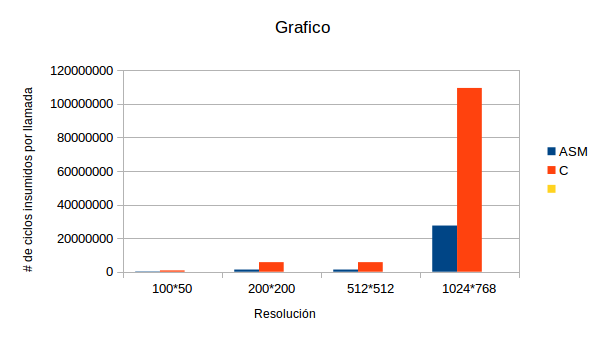
\includegraphics[scale=1]{temperature.png}
 \end{center}
  \vspace*{0.3cm} 
La diferencia principal entre el c\'odigo escrito en lenguaje C y el c\'odigo ASM, es la cantidad de accesos 
a memoria realizados en cada iteraci\'on. Otra diferencia puede verse en la cantidad de bytes que pueden 
ser procesados simultaneamente durante el mismo ciclo. 
Mientras que en C leemos y procesamos un byte por vez, el c\'odigo ASM nos permite acceder y procesar 
16 bytes en simultaneos. De todas maneras, en este caso trabajamos con 12 bytes que es un numero mas \'util 
ya que es m\'ultiplo de 3 (cantidad de bytes por p\'ixel)  y de 4 (cantidad de bytes por cada caracter).
Pudiendo levantar de a 16 bytes en memoria, podr\'ia esperarse que el c\'odigo asm demorase una 
diesiseiava parte de la cantidad de ciclos que demora el c\'odigo en C.
Pero debemos tener en cuenta que en nuestro caso estamos aprovechando solo 15 de los 16 bytes que leemos 
en cada iteraci\'on por lo tanto es más acertado evaluar como si solo leyeramos 15 bytes. 
Adem\'as, hay que tener en cuenta que las instrucciones SSE pueden necesitar más ciclos que las operaciones 
comunes que usamos en el C, eso disminuye un poco la performance en la comparación. 
\vspace*{0.3cm} \vspace*{0.3cm} 
 %Luego de dichas mediciones podemos concluir en que la implementacion en ASM por el uso del 
 %paralelismo con instrucciones sse posee una mejor performance.
 %Además teniendo en cuenta que los accesos a memoria son muy costosos, 
 %el paralelismo hace que se reduzcan estos mismos.
 
 
\newpage

\subsection{Filtro LDR}

\vspace*{0.3cm} \noindent
\subsubsection{Objetivo}

El objevtivo de este filtro, es tomar una imagen y transformar el color, pero dándole un efecto de iluminación. \newline
Para lograrlo, se toma el valor de un pixel y le agrega un porcentaje alfa de sus pixels vecinos. \newline
Si ese porcentaje es positivo, los pixels claros, se vuelven aún más claros y los oscuros se mantienen igual.\newline

%\[ dst_{(x,y)} = \left\{ \begin{array}{ll}
%        src_{(i,j)} & \mbox{si $i < 2 \vee j < 2 \vee i + 2 \leq tamy \vee j + 2 \leq tamx $}\\
%       pepe & \mbox{si no}\\\\end{array} \right. \]
       
\[ dst_{(i,j)} = \left\{ \begin{array}{ll}
         src_{(i,j)} & \mbox{si $i < 2 \vee j < 2 \vee i + 2 \leq tamy \vee j + 2 \leq tamx  $}\\
        min(max(src_{(i,j)} + var_{(i,j)},0, 255)) & \mbox{si no}\\\end{array} \right. \]     
        
Donde:

$var (i,j) = \frac{src(i, j) * \alpha * sumargb (i,j)}{max}$ \newline

Donde:\newline

$sumargb_{(i,j)} = suma_r{(i,j)} + suma_{g(i,j)} + suma_{b(i,j)}$ \newline

$max = 5 * 5 * 255 * 3 * 255$\newline

Y suma\_r suma\_g y suma\_b es la suma de los pixeles vecinos desde $-2 \leq i \leq 2$ y $-2 \leq j \leq 2$

\vspace*{0.3cm} \noindent

\subsubsection{Desarrollo Implementacion C}

\begin{center}
\textbf{Sintesis de Desarrollo} 
\end{center}

Recorremos la totalidad de la imagen fuente mediante 2 ciclos, uno para filas, y otro para columnas.
Dentro de esta iteración, hacemos dos cosas: en los bordes (de dos pixels) copiamos la imagen fuente en destino tal cual.
Por otra parte, procesamos la parte central que no es borde. Para procesar este centro, tomamos cada pixel y calculamos la 
sumargb con 2 ciclos también. Al obtener esa suma, seguimos con lo indicado en el enunciado, multiplicamos por alfa y dividimos
por max. \newline
Finalmente, para pegar el valor final en el pixel de la imagen destino, hacemos un máximo y un mínimo, 
para que el valor quede entre 0 y 255.


%\newline

\begin{center}
\textbf{Explicación detallada de Implementación}

\end{center}

En esta implementación, inicialmente,se crearon dos punteros de matriz uno correspondiente a src y otro a dst.\newline 
Ademas, 4 enteros llamados $sumargb$, $varr$,$varg$ y $varb$ inicializados en 0 y otro entero $max$ inicializado en 4876875. \newline
Luego, realizamos dos ciclos, uno añidado dentro del otro recorriendo de la forma $'(int\ i = 0;\ i < filas;\ i++)'$ y 
$(int\ j = 0;\ j < cols;\ j\ ++)$.\newline
Dentro del segundo ciclo, creamos dos punteros rgb\_t donde uno apuntará a \newline rgb\_t $*p\_d = (rgb\_t*)\  \&dst\_matrix[i][j*3]$, y el otro
a $rgb\_t *p\_s = (rgb\_t*)\ \&src\_matrix[i][j*3]$.\newline
Posteriormente, chequeamos si nos encontramos recorriendo los bordes de la imagen \newline $(i < 2 || j < 2 || (i + 2) >= filas || (j + 2) >= cols)$,
en caso verdadero, guardamos el puntero p\_s en p\_d $*p_d=*p_s$. \newline
En caso negativo, realizamos lo siguiente:\newline
Primero guardamos en $sumargb$ el valor 0, luego, crearemos dos ciclos, uno añidado del otro recorriendo de la siguiente forma:\newline
$(int\  i\_p = i-2;\  i\_p <= i+2;\  ++i\_p)$ $(int\  j\_p = j-2;\  j\_p <= j+2;\  ++j\_p)$, dentro del ciclo interno,
creamos un rgb\_t $rgb\_t *s\_s = (rgb\_t*)\  \&src\_matrix[i\_p][j\_p*3]$ y posteriormente al entero $sumargb$ le almacenamos la
suma entre los valores r, g y b del rgb\_t s\_s.\newline
Fuera de estos dos ciclos, y aun dentro de la parte falsa del if, realizamos las siguientes operaciones:\newline
Primero, al entero $varb$ le almacenamos el valor b del rgb\_t p\_s multiplicado por $alfa$ (dado como parametro) y por $sumargb$ $varb = (p\_s\rightarrow b * alfa * sumargb);$.\newline
Segundo, al entero $varg$ le almacenamos el valor g del rgb\_t p\_s multiplicado por $alfa$ (dado como parametro) y por $sumargb$ $varg = (p\_s\rightarrow g * alfa * sumargb);$.\newline
Tercero, al entero $varr$ le almacenamos el valor r del rgb\_t p\_s multiplicado por $alfa$ (dado como parametro) y por $sumargb$ $varr = (p\_s\rightarrow r * alfa * sumargb);$.\newline
Luego, a cada uno de estos tres enteros los dividimos por $max$: \newline
$varb = varb/max;
varg = varg/max;
varr = varr/max;$\newline
Y, por ultimo, al valor b del rgb\_t p\_d le almacenamos $MIN(MAX(p\_s\rightarrow b + varb, 0),255)$ donde MIN y MAX son funciones dadas por la catedra, \newline
Al valor g del rgb\_t p\_d le almacenamos $MIN(MAX(p\_s\rightarrow g + varg, 0),255)$,\newline
Al valor r del rgb\_t p\_d le almacenamos $MIN(MAX(p\_s\rightarrow r + varr, 0),255)$.\newline
Damos por finalizada la parte falsa del if.\newline

Estos dos ciclos realizaran $j\_d = cols - 1$  por $i\_d = filas -1$ de itereaciones.\newline
Con lo mencionado, obtenemos el filtro temperature en c correctamente, con los valores que nos pasan como parámetros.\newline

\vspace*{0.3cm} \noindent
\subsubsection{Desarrollo Implementacion en ASM}
En esta implementacion, a diferencia de en Popart y Temperature, no hubieron tantos casos por chequear, sino que trabajamos 
los bordes por un lado, y la parte interna por el otro. \newline
Recorrimos, por columna de la siguiente forma: \newline

$\hspace*{2.2cm}$$mov\  R12D, 0 $\newline$
$\hspace*{2.8cm}$mov\  R13D, 0 $\newline$
$\hspace*{2.8cm}$mov\  R14D, 0 $\newline$
$\hspace*{2.8cm}$mov\  EBX, 0 $\newline$
$\hspace*{2.8cm}$.recorrido\_fila:$\newline$
$\hspace*{2.8cm}$cmp\  R13D, EDX $\newline$
$\hspace*{2.8cm}$je\  .fin$\newline$
$\newline$
$\hspace*{2.8cm}$.recorrido\_columna:$\newline$
$\hspace*{2.8cm}$	cmp\  R12D, ECX $\newline$
$\hspace*{2.8cm}$	je\  .siguiente\_columna$\newline$
$\newline$
$\hspace*{2.8cm}; me fijo si es borde o interior\newline$
$\hspace*{2.8cm}$cmp\  R12D, 2$\newline$
$\hspace*{2.8cm}$jl\  .es\_borde$\newline$
$\hspace*{2.8cm}$cmp\  R13D, 2$\newline$
$\hspace*{2.8cm}$jl\  .es\_borde$\newline$
$\hspace*{2.8cm}$mov\  EAX, R12D $\newline$
$\hspace*{2.8cm}$add\  EAX, 2$\newline$
$\hspace*{2.8cm}$cmp\  EAX, ECX $\newline$
$\hspace*{2.8cm}$jge\  .es\_borde$\newline$
$\hspace*{2.8cm}$mov\  EAX, R13D $\newline$
$\hspace*{2.8cm}$add\  EAX, 2$\newline$
$\hspace*{2.8cm}$cmp\  EAX, EDX$\newline$
$\hspace*{2.8cm}$jge\  .es\_borde$\newline

Inicializamos varios registros en 0 y comparamos si es Menor a 2 la fila y/o la columna, y en caso de ser asi, chequeamos los
bordes así:

$.es\_borde: ; copio la misma imagen$\newline$
$\hspace*{2.8cm}$	xor\  RAX, RAX$\newline$
$\hspace*{2.8cm}$	mov\  EAX, EBX$\newline$
$\hspace*{2.8cm}$	add\  EAX, R14D$\newline$
$\hspace*{2.8cm}$	mov\  R15, [RDI + RAX]$\newline$
$\hspace*{2.8cm}$	mov\  [RSI + RAX], R15D$\newline$
$\newline$
$\hspace*{2.8cm}$.seguir:$\newline$
$\hspace*{2.8cm}$add\  R12D, 1$\newline$
$\hspace*{2.8cm}$add\  R14D, R8D$ ; R14D = R14D + src\_row\_size\newline$
$\hspace*{2.8cm}$jmp\  .recorrido_columna$$\newline$

Estas iteraciones se realizaran hasta que R12D y R13D sean mayores a 2. \newline
Una vez que esto ocurre pasamos a sumar cada color haciendo:\newline

$\hspace*{2.2cm}$$movdqu\  XMM7, XMM0 $\newline$
$\hspace*{2.8cm}$movdqu\  XMM8, XMM0 $\newline$
$\hspace*{2.8cm}$xorpd\  XMM9, XMM9 $\newline$
$\newline$
$\hspace*{2.8cm}$pshufb\  XMM0, [MASK\_1\_COLOR]$\newline$
$\hspace*{2.8cm}$movdqu\  XMM10, XMM0$\newline$
$\hspace*{2.8cm}$punpcklbw\  XMM10, XMM9 $\newline$
$\hspace*{2.8cm}$pshufb\  XMM7, [MASK\_1\_COLORGREEN]$\newline$
$\hspace*{2.8cm}$movdqu\  XMM12, XMM7$\newline$
$\hspace*{2.8cm}$punpcklbw\  XMM12, XMM9$\newline$
$\hspace*{2.8cm}$pshufb\  XMM8, [MASK\_1\_COLORBLUE] $\newline$
$\hspace*{2.8cm}$movdqu\  XMM14, XMM8$\newline$
$\hspace*{2.8cm}$punpcklbw\  XMM14, XMM9 $\newline$
$\hspace*{2.8cm}$paddw\  XMM10, XMM12$\newline$
$\hspace*{2.8cm}$paddw\  XMM10, XMM14$\newline$
$\hspace*{2.8cm}$movdqu\  XMM0, XMM10$\newline
\newline
Primero, nos guardamos en XMM0 los primeros 15 pixeles haciendo $ movdqu\  XMM0, [RDI]$, luego, el valor de XMM0,
lo guardamos en XMM7 y XMM8, limpiamos XMM9 y con 3 mascaras distintas que lo que hacen es ponernos los 5 pixeles rojos adelante y llenar con 0, 
los 5 pixeles azules y llenar con cero y los 5 pixeles verdes y llenar con ceros. \newline
Realizamos la operacion Pshufb con los tres xmm y las mascaras (un xmm con cada mascara) y luego desempaquetamos de byte a word,
usando el XMM9 que habiamos llenado de 0. \newline
El desempaquetado hace que nos queden los valores en word en los registros XMM10, XMM12, XMM14 respectivamente, y luego
los sumamos con PADDW guardando el valor en XMM10. De esta forma obtenemos en word 
$|b0 + g0 + r0|b1 + g1 + r1|b2 + g2 + r2|b3 + g3 + r3|b4 + g4 + r4|$. \newline
Esto lo realizamos 5 veces, quedandonos con los valores en XMM1, 2 ,3,4 y 5. Luego, sumamos estos XMM y nos queda
el valor en XMM3. Proximo a esto, procedemos a sumar los vecinos: \newline

$\hspace*{2.3cm}$$movdqu\ XMM8,\ XMM3$\newline$
$\hspace*{2.8cm}$movdqu\ XMM9,\ XMM3 $\newline$
$\hspace*{2.8cm}$psrldq XMM9, 8D$\newline$
$\hspace*{2.8cm}$paddw\ XMM3,\ XMM9$\newline$
$\newline$
$\hspace*{2.8cm}$movdqu\ XMM9,\ XMM8 $\newline$
$\hspace*{2.8cm}$psrldq XMM9, 6D$\newline$
$\hspace*{2.8cm}$paddw\ XMM3,\ XMM9$\newline$
$\hspace*{2.8cm}$movdqu\ XMM9,\ XMM8$\newline$
$\hspace*{2.8cm}$psrldq XMM9, 4D$\newline$
$\hspace*{2.8cm}$paddw\ XMM3,\ XMM9$\newline$
$\newline$
$\hspace*{2.8cm}$movdqu\ XMM9,\ XMM8 $\newline$
$\hspace*{2.8cm}$psrldq\  XMM9, 2D$\newline$
$\hspace*{2.8cm}$paddw\ XMM3,\ XMM9$\newline$
$\hspace*{2.8cm}$movdqu\ XMM9,\ XMM3$\newline$
$\hspace*{2.8cm}$psrldq\  XMM9, 2D$\newline$
$\hspace*{2.8cm}$pslldq\  XMM9, 2D$\newline$
$\hspace*{2.8cm}$psubw\ XMM3,\ XMM9 $\newline

En esta seccion vamos moviendo bytes a la izquierda, 8 6 4 y 2 asi logramos sumar todos los vecinos en los packs.\newline
Guardamos en R15D el valor alfa, que nos viene por pila en $[RSP + 56]$. Y lo guardamos en XMM15\newline
Procedemos a la multiplicación por alfa:\newline

$\hspace*{2.3cm}$$movdqu\ XMM7,\ XMM3$\newline$
$\hspace*{2.8cm}$xorpd\ XMM9,\ XMM9$\newline$
$\hspace*{2.8cm}$punpcklwd\ XMM7,\ XMM9$\newline$
$\hspace*{2.8cm}$cvtdq2pd\ XMM7,\ XMM7$\newline$
$\hspace*{2.8cm}$cvtdq2pd\ XMM15,\ XMM15$\newline$
$\hspace*{2.8cm}$mulpd XMM7,\ XMM15$\newline$
$\hspace*{2.8cm}$cvtpd2Dq\ XMM7,XMM7$\newline$
$\hspace*{2.8cm}$movdqu\ XMM3,\ XMM7$$\newline$

En esta seccion desempaquetamos de WORD a DWORD y convertimos a Double para multiplicar con alfa, luego lo convertimos a DWORD.
Guardamos en XMMO el valor de XMM6 y nos quedamos con el del medio, por consiguiente pasamos a multiplicar lo que tenemos con SUMARGB 
y dividimos por MAX: \newline

$\hspace*{2.3cm}$$movdqu XMM7, XMM0$\newline$
$\hspace*{2.8cm}$	movdqu XMM8, XMM0 $\newline$
$\hspace*{2.8cm}$	$\newline$
$\hspace*{2.8cm}$	cvtdq2pd\ XMM3,\ XMM3$\newline$
$\newline$
$\hspace*{2.8cm}$	xorpd\  XMM9, XMM9 $\newline$
$\hspace*{2.8cm}	;multiplico blue \newline$
$\hspace*{2.8cm}$	pshufb\  XMM0, [MASK\_1\_COLOR] $\newline$
$\hspace*{2.8cm}$	movdqu\  XMM10, XMM0$\newline$
$\hspace*{2.8cm}$	punpcklbw\  XMM10, XMM9$\newline$
$\hspace*{2.8cm}$	movdqu\ XMM13, XMM10$\newline$
$\hspace*{2.8cm}$	xorpd\ XMM9,\ XMM9$\newline$
$\hspace*{2.8cm}$	punpcklwd\ XMM13,\ XMM9$\newline$
$\hspace*{2.8cm}$	cvtdq2pd\ XMM13,\ XMM13$\newline$
$\hspace*{2.8cm}$	mulpd\ XMM13,\ XMM3$\newline$
$\hspace*{2.8cm}$	movdqu\  XMM1, XMM13$\newline$
$\newline$
$\hspace*{2.8cm}	;multiplico verde
\newline$
$\hspace*{2.8cm}$	pshufb\  XMM7, [MASK\_1\_COLORGREEN] $\newline$
$\hspace*{2.8cm}$	movdqu\  XMM11, XMM7$\newline$
$\hspace*{2.8cm}$	punpcklbw\  XMM11, XMM9$\newline$
$\hspace*{2.8cm}$	$\newline$
$\hspace*{2.8cm}$	movdqu\ XMM13, XMM11$\newline$
$\hspace*{2.8cm}$	xorpd\ XMM9,\ XMM9 $\newline$
$\hspace*{2.8cm}$	punpcklwd\ XMM13,\ XMM9$\newline$
$\hspace*{2.8cm}$	cvtdq2pd\ XMM13,\ XMM13$\newline$
$\newline$
$\hspace*{2.8cm}$	mulpd\ XMM13,\ XMM3$\newline$
$\newline$
$\hspace*{2.8cm}$	movdqu XMM5, XMM13$\newline$
$\newline$
$\hspace*{2.8cm}	;multiplico red\newline$
$\hspace*{2.8cm}$	pshufb\  XMM8, [MASK\_1\_COLORBLUE]$\newline$
$\hspace*{2.8cm}$	movdqu\  XMM12, XMM8$\newline$
$\hspace*{2.8cm}$	punpcklbw\  XMM12, XMM9$\newline$
$\hspace*{2.8cm}$	movdqu\ XMM13, XMM12$\newline$
$\newline$
$\hspace*{2.8cm}$	xorpd\ XMM9,\ XMM9$\newline$
$\hspace*{2.8cm}$	punpcklwd\ XMM13,\ XMM9$\newline$
$\hspace*{2.8cm}$	cvtdq2pd\ XMM13,\ XMM13$\newline$
$\hspace*{2.8cm}$	mulpd\ XMM13,\ XMM3$\newline$
$\hspace*{2.8cm}$	movdqu\  XMM7, XMM13$\newline

En esta parte procedemos a realizar la multiplicacion de cada color por separado con lo que ya teniamos. Desempaquetando,
convirtiendo a double y por finalizado multiplicando quedandonos en el XMM1, 5 Y 7 los valores obtenidos.\newline
Luego, realizamos la division por max:\newline

$\hspace*{2.3cm}$$ movdqu\  XMM11, [MASK\_MAX]$\newline$
$\hspace*{2.8cm}$cvtdq2pd\  XMM11,XMM11$\newline$
$\hspace*{2.8cm}$divpd\  XMM1, XMM11 $\newline$
$\hspace*{2.8cm}$cvttpd2Dq\  XMM1,XMM1 $\newline$
$\hspace*{2.8cm}$packssdw\  XMM1, XMM1$\newline$
$\hspace*{2.8cm}$;GREEN$\newline$
$\hspace*{2.8cm}$divpd\ XMM5,XMM11 $\newline$
$\hspace*{2.8cm}$cvttpd2Dq\ XMM5,XMM5$\newline$
$\hspace*{2.8cm}$packssdw\ XMM5,\ XMM5$\newline$
$\hspace*{2.8cm}$;rojo$\newline$
$\hspace*{2.8cm}$divpd\ XMM7,XMM11 $\newline$
$\hspace*{2.8cm}$cvttpd2Dq\ XMM7,XMM7$\newline$
$\hspace*{2.8cm}$packssdw\ XMM7,\ XMM7$\newline$
$\newline$
$\hspace*{2.8cm}$movdqu\ XMM9,\ XMM1$\newline$
$\hspace*{2.8cm}$psrldq\  XMM9, 2D$\newline$
$\hspace*{2.8cm}$pslldq\  XMM9, 2D$\newline$
$\hspace*{2.8cm}$psubw\ XMM1,\ XMM9 ;resto para q no me quede basura
$\newline$
$\hspace*{2.8cm}$movdqu\ XMM9,\ XMM5$\newline$
$\hspace*{2.8cm}$psrldq\  XMM9, 2D$\newline$
$\hspace*{2.8cm}$pslldq\  XMM9, 2D$\newline$
$\hspace*{2.8cm}$psubw\ XMM5,\ XMM9 ;resto para q no me quede basura
$\newline$
$\hspace*{2.8cm}$movdqu\ XMM9,\ XMM7$\newline$
$\hspace*{2.8cm}$psrldq\  XMM9, 2D$\newline$
$\hspace*{2.8cm}$pslldq\  XMM9, 2D$\newline$
$\hspace*{2.8cm}$psubw\ XMM7,\ XMM9 ;resto para q no me quede basura
$\newline$
$\hspace*{2.8cm}$;en\ XMM1 tengo blue$\newline$
$\hspace*{2.8cm}$;en\ XMM5 tengo GREEN$\newline$
$\hspace*{2.8cm}$;en\ XMM7 tengo rojo$\newline$
$\hspace*{2.8cm}$; en\ XMM6 me quede con el actual$\newline$
$\hspace*{2.8cm}$movdqu\ XMM15,\ XMM6$\newline$
$\hspace*{2.8cm}$pshufb\ XMM15, [MEQUEDOCONELDELMEDIO]$\newline$
$\hspace*{2.8cm}$movdqu\ XMM8,\ XMM15$\newline$
$\hspace*{2.8cm}$movdqu\ XMM9,\ XMM15$\newline$
$\hspace*{2.8cm}$movdqu\ XMM10,\ XMM15$\newline$
$\hspace*{2.8cm}$pshufb\ XMM8, [MASKCOLORROJO] $\newline$
$\hspace*{2.8cm}$paddw\ XMM8,\ XMM1$\newline$
$\hspace*{2.8cm}$pshufb\ XMM9, [MASKCOLORVERDE]$\newline$
$\hspace*{2.8cm}$paddw\ XMM9,\ XMM5$\newline$
$\hspace*{2.8cm}$pshufb\ XMM10, [MASKCOLORAZUL]$\newline$
$\hspace*{2.8cm}$paddw\ XMM10,\ XMM7$\newline

En esta seccion realizamos la division por max, a diferencia de las otras conversiones, en esta convertimos truncado a double
para no perder presicion en la division. Luego de dividir realizamos distintos shifteos, y proximo a esto, shufteos con mascaras
para ir quedandonos definitivamente con cada color final y sumandolos entre si para proceder a chequear maximos y minimos.\newline
El resultado final lo tenemos en XMM8,9 y 10.\newline

Pasamos a chequear dichos valores:\newline
Primero, chequeando si es mayor a cero: \newline

$\hspace*{2.3cm}$$movdqu\  XMM14,[M0]$\newline$
$\hspace*{2.8cm}$movdqu\ XMM15,XMM0$\newline$
$\hspace*{2.8cm}$pcmpgtw\  XMM15, XMM14$$\newline$

Donde, M0 es una mascara con todos 0. \newline

Y procedemos a:\newline

$\hspace*{2.3cm}$$movdqu\  XMM13,\ XMM0$\newline$
$\hspace*{2.8cm}$	movdqu\ XMM11,\ XMM15  ;$\newline$
$\hspace*{2.8cm}$	pcmpeqw\  XMM14,XMM14 $\newline$
$\hspace*{2.8cm}$	pxor\ XMM11,\ XMM14$\newline$
$\hspace*{2.8cm}$	movdqu\ XMM2, [M0]$\newline$
$\hspace*{2.8cm}$	pand\ XMM2,XMM11$\newline$
$\hspace*{2.8cm}$	pand\ XMM13,\ XMM15$\newline$
$\hspace*{2.8cm}$	movdqu\ XMM1,\ XMM13$\newline

Esto, similar a nuestros chequeos en las implementaciones anteriores de Popart y Temperature, guardamos el valor de la comparación,
realizamos and con los valores chequeados, invertimos el resultado de la comparacion y lo guardamos para que esos casos no vuelvan
a ser chequeados. Luego, nuestro resultado nos queda en XMM1. \newline

Segundo, si el numero es menor a 255: \newline

$\hspace*{2.3cm}$$orpd\ XMM1,XMM2$\newline$
$\hspace*{2.8cm}$movdqu\ XMM0,\ XMM1$\newline$
$\hspace*{2.8cm}$movdqu\  XMM14,[M255]$\newline$
$\hspace*{2.8cm}$movdqu\ XMM15,XMM0$\newline$
$\hspace*{2.8cm}$pcmpgtw XMM14,XMM15$\newline

Donde, M255 es una mascara con todos 255. \newline$\hspace*{2.8cm}$

Procedemos a:\newline

$\hspace*{2.3cm}$$movdqu XMM13,\ XMM0$\newline$
$\hspace*{2.8cm}$	movdqu\ XMM11,\ XMM14  $\newline$
$\hspace*{2.8cm}$	pcmpeqw\  XMM15,XMM15 $\newline$
$\hspace*{2.8cm}$	pxor\ XMM11,\ XMM15$\newline$
$\hspace*{2.8cm}$	movdqu\ XMM4, [M255]$\newline$
$\hspace*{2.8cm}$	pand\ XMM4,XMM11$\newline$
$\hspace*{2.8cm}$	pand\ XMM13,\ XMM14$\newline$
$\hspace*{2.8cm}$	movdqu\ XMM3,\ XMM13$\newline

Esta seccion, como mencionamos antes, similar a las implementaciones anteriores, guardamos el valor de la comparación,
realizamos and con los valores chequeados, invertimos el resultado de la comparacion y lo guardamos para que esos casos no vuelvan
a ser chequeados. Luego, nuestro resultado nos queda en XMM3. \newline

Por ultimo, en nuestra implementacion, juntamos los resultados, chequeando con un contador si pertenece a verde rojo o todo:\newline

$\hspace*{2.3cm}$$add\  r15, 1$\newline$
$\hspace*{2.8cm}$orps\ XMM3,XMM4$\newline$
$\hspace*{2.8cm}$movdqu\ XMM0,XMM3$\newline$
$\hspace*{2.8cm}$cmp\  r15,1$\newline$
$\hspace*{2.8cm}$je\  .verdes$\newline$
$\hspace*{2.8cm}$cmp\  r15,2$\newline$
$\hspace*{2.8cm}$je\  .rojos$\newline$
$\hspace*{2.8cm}$cmp\  r15,3$\newline$
$\hspace*{2.8cm}$je\  .juntoTodo$$\newline$

$.verdes:$\newline$
$\hspace*{2.8cm}$movdqu\ XMM8,\ XMM0$\newline$
$\hspace*{2.8cm}$movdqu\ XMM0,\ XMM9$\newline$
$\hspace*{2.8cm}$jmp\  .chequeo$\newline$
$\hspace*{2.8cm}$\ 	.rojos:$\newline$
$\hspace*{2.8cm}$movdqu\ XMM9,\ XMM0$\newline$
$\hspace*{2.8cm}$movdqu\ XMM0,\ XMM10$\newline$
$\hspace*{2.8cm}$jmp\  .chequeo$\newline$
$\hspace*{2.8cm}$\ 	.juntoTodo:$\newline$
$\hspace*{2.8cm}$movdqu\ XMM10,\ XMM0$\newline$
$\hspace*{2.8cm}$pslldq\ XMM9, 1d$\newline$
$\hspace*{2.8cm}$pslldq\ XMM10, 2D$\newline$
$\hspace*{2.8cm}$paddb\ XMM8,\ XMM9$\newline$
$\hspace*{2.8cm}$paddb\ XMM8,\ XMM10$\newline$
$\hspace*{2.8cm}$movdqu\ XMM0,\ XMM8$\newline

En esta seccion, como mencionamos, realizamos la suma de todos los xmm de los distintos colores.\newline
Una ves terminado esto, guardamos en la imagen resultante los valores: \newline

\hspace*{2.3cm}$xor\  RAX, RAX$\newline$
$\hspace*{2.8cm}$mov\  EAX, EBX$\newline$
$\hspace*{2.8cm}$add\  EAX, R14D$\newline$
$\hspace*{2.8cm}$xor\  R15, R15$\newline$
$\hspace*{2.8cm}$movd\  R15D, XMM0$\newline$
$\hspace*{2.8cm}$mov\  [RSI + RAX], R15D$$\newline$

Esto, finalmente, se realizará hasta que no queden columnas y filas por verse.



\vspace*{0.3cm} \noindent
\subsubsection{Experimento 1}

  Analizar cuales son las diferencias de performace entre las versiones de C y ASM. 
  Realizar gráficos que representen estas diferencias.
  
\vspace*{0.3cm} \noindent

 En este filtro a diferencia de los anteriores existe un alfa el cual da valores positivos y negativos,
 por ende realizamos mediciones con alfa positivo y negativo.
 \vspace*{0.3cm} \noindent
 
 Realizando nuestras mediciones en la implementacion de C y de ASM de nuestro codigos con alfa positivo 
 obtenemos para disversas resoluciones: \vspace*{0.3cm} \noindent
 
 
 120x56
 
En ASM: 1460376

En C:3431854

 \vspace*{0.3cm} \noindent
200x200

En ASM: 9112044

En C:21743294

 \vspace*{0.3cm} \noindent
512x512

En ASM: 64050524

En C:145683856

 \vspace*{0.3cm} \noindent
1023x767

En ASM :193531520

En C:438512256


  \vspace*{0.3cm}

 Para una mejor representación se realizo un grafico mostrando a simple vista
 las diferencias entre cada tipo de implementacion con dicho alfa.
 \vspace*{0.3cm} \vspace*{0.3cm}
  \begin{center}
 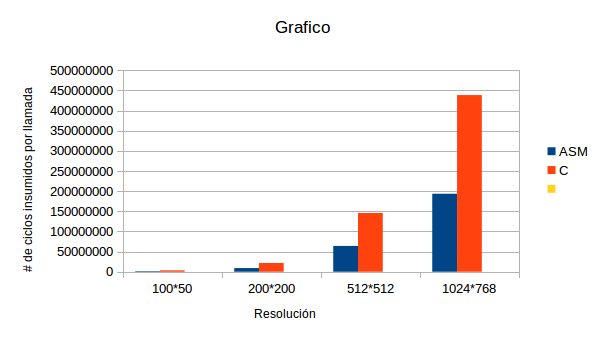
\includegraphics[scale=1]{ldr+.png}
 \end{center}
  \vspace*{0.3cm} 

  Por consiguiente, con un valor alfa negativo realizamos las pertinentes mediciones en las distintas implementaciones 
  obteniendo que: \vspace*{0.3cm} \noindent
  
  
  120x56
  
En ASM: 1438545

En C:3450531

 \vspace*{0.3cm} \noindent
200x200

En ASM: 9026611

En C:21783128

 \vspace*{0.3cm} \noindent
512x512

En ASM: 63927320

En C:145574048

 \vspace*{0.3cm} \noindent
1023x767

En ASM: 193388816

En C:437996160


  
  \vspace*{0.3cm}

 Para una mejor representación se realizo un grafico mostrando a simple vista
 las diferencias entre cada tipo de implementacion con dicho alfa.
 \vspace*{0.3cm} \vspace*{0.3cm}
  \begin{center}
 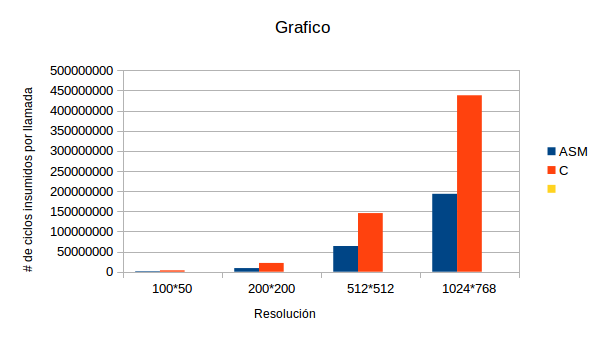
\includegraphics[scale=1]{ldr-.png}
 \end{center}
  \vspace*{0.3cm} 
  
  
La diferencia principal entre el c\'odigo escrito en lenguaje C y el c\'odigo ASM, es la cantidad de accesos 
a memoria realizados en cada iteraci\'on.Otra diferencia puede verse en la cantidad de bytes que pueden 
ser procesados simultaneamente durante el mismo ciclo. En nuestra implamentacion de ASM en una sola iteracion ya
obtenemos la sumas correspondientes de los pixeles vecinos, mientras que en la implamentacion del c por cada iteracion
se realizan dentro de esa misma varias iteraciones mas sumando los pixeles vecinos y por este motivo principal
la diferencia notoria en la performance.\vspace*{0.2cm}

Pudiendo levantar de a 16 bytes en memoria, podr\'ia esperarse que el c\'odigo asm demorase una 
diesiseiava parte de la cantidad de ciclos que demora el c\'odigo en C.
Pero debemos tener en cuenta que en nuestro caso estamos aprovechando solo 15 de los 16 bytes que leemos 
en cada iteraci\'on por lo tanto es más acertado evaluar como si solo leyeramos 15 bytes. 
Adem\'as, hay que tener en cuenta que las instrucciones SSE pueden necesitar más ciclos que las operaciones 
comunes que usamos en el C, eso disminuye un poco la performance en la comparación. 
\vspace*{0.3cm} \vspace*{0.3cm} 

\newpage


%%%%%%%%%%%%%%%%%%%%%%%%%%%%%%%%%%%%%%%%%%%%%%%%%%%%%%%%%%%%%%%%%%%%%%%%%%%%%%%
%% Conclusión                                                                %%
%%%%%%%%%%%%%%%%%%%%%%%%%%%%%%%%%%%%%%%%%%%%%%%%%%%%%%%%%%%%%%%%%%%%%%%%%%%%%%%

\newpage
\section{Conclusión}

Las instrucciones SIMD (Single Instruction Multiple Data) proveen al programador de una herramienta más efectiva para realizar el mismo conjunto de operaciones a una gran cantidad de datos.

La aplicación de filtros a imágenes era un ejemplo perfecto para probar su eficiencia.

Analizando los resultados de las implementaciones de los 3 filtros, podemos notar:

\begin{itemize}
\item Las operaciones básicas (padd, psub, pmul, pdiv, shifts, etc.) SIMD tienen un costo similar a sus correspondientes operaciones unitarias, pero generalmente requieren algún tipo de pre-proceso para poder trabajar con los 16 bytes (pack, unpack, shifts) en una sola iteración, por lo tanto, aunque más eficientes, no lo son en una relación directamente proporcional.
\item En el caso que sí hay una relación directamente proporcional es en el acceso a memoria.
\item Además, el acceso a memoria es, por lejos, la operación más costosa de las que implementamos en cada filtro.
\item Por consecuencia directa del ítem anterior, las llamadas a otras funciones (que a su vez, probablemente contengan variable locales) dentro de una iteración provocan estragos en la efectividad de las implementaciones en C.
\item Para poder aprovechar las instrucciones SIMD es un prerequisito que los datos estén contiguos en memoria.
\end{itemize}

Concluimos que, definitivamente, las instrucciones SIMD, cuando pueden aprovecharse, demuestran una gran eficiencia. Sin embargo, hay que tener algunas consideraciones:

Aunque las imágenes, video y sonido son los primeros candidatos a ser optimizados por paralelización, no todos los procesos pueden ser efectivos y se requiere un análisis profundo de los datos para ver si vale el esfuerzo.

Además, aunque se pueda lograr una gran optimización, no siempre es lo más importante. La optimización seguramente es indispensable en transmisiones de video en vivo, pero baja en importancia si tuviese que ser aplicado una sola vez en una aplicación tipo MS Paint.

Las desventajas que podrían opacar a la optimización son:

El código no es portable, únicamente funciona en procesadores que implementan el set de instrucciones AMD64, requiriendo reescrituras para otras plataformas. Sin embargo el código C debería funcionar perfectamente en IA-32, ARM y cualquier otro procesador que tenga un compilador de lenguaje C.

El código es mucho más largo y difícil de entender (por lo tanto mayor posibilidad de tener bugs) que en un lenguaje de más alto nivel como C. Y en pos de la optimización, se llegan a eliminar funciones (poniéndolas inline), lo que genera código repetido, largo y confuso.




\end{document}
